\documentclass[twoside]{book}

% Packages required by doxygen
\usepackage{fixltx2e}
\usepackage{calc}
\usepackage{doxygen}
\usepackage[export]{adjustbox} % also loads graphicx
\usepackage{graphicx}
\usepackage[utf8]{inputenc}
\usepackage{makeidx}
\usepackage{multicol}
\usepackage{multirow}
\PassOptionsToPackage{warn}{textcomp}
\usepackage{textcomp}
\usepackage[nointegrals]{wasysym}
\usepackage[table]{xcolor}

% NLS support packages
\usepackage[french]{babel}

% Font selection
\usepackage[T1]{fontenc}
\usepackage[scaled=.90]{helvet}
\usepackage{courier}
\usepackage{amssymb}
\usepackage{sectsty}
\renewcommand{\familydefault}{\sfdefault}
\allsectionsfont{%
  \fontseries{bc}\selectfont%
  \color{darkgray}%
}
\renewcommand{\DoxyLabelFont}{%
  \fontseries{bc}\selectfont%
  \color{darkgray}%
}
\newcommand{\+}{\discretionary{\mbox{\scriptsize$\hookleftarrow$}}{}{}}

% Page & text layout
\usepackage{geometry}
\geometry{%
  a4paper,%
  top=2.5cm,%
  bottom=2.5cm,%
  left=2.5cm,%
  right=2.5cm%
}
\tolerance=750
\hfuzz=15pt
\hbadness=750
\setlength{\emergencystretch}{15pt}
\setlength{\parindent}{0cm}
\setlength{\parskip}{3ex plus 2ex minus 2ex}
\makeatletter
\renewcommand{\paragraph}{%
  \@startsection{paragraph}{4}{0ex}{-1.0ex}{1.0ex}{%
    \normalfont\normalsize\bfseries\SS@parafont%
  }%
}
\renewcommand{\subparagraph}{%
  \@startsection{subparagraph}{5}{0ex}{-1.0ex}{1.0ex}{%
    \normalfont\normalsize\bfseries\SS@subparafont%
  }%
}
\makeatother

% Headers & footers
\usepackage{fancyhdr}
\pagestyle{fancyplain}
\fancyhead[LE]{\fancyplain{}{\bfseries\thepage}}
\fancyhead[CE]{\fancyplain{}{}}
\fancyhead[RE]{\fancyplain{}{\bfseries\leftmark}}
\fancyhead[LO]{\fancyplain{}{\bfseries\rightmark}}
\fancyhead[CO]{\fancyplain{}{}}
\fancyhead[RO]{\fancyplain{}{\bfseries\thepage}}
\fancyfoot[LE]{\fancyplain{}{}}
\fancyfoot[CE]{\fancyplain{}{}}
\fancyfoot[RE]{\fancyplain{}{\bfseries\scriptsize Généré par Doxygen }}
\fancyfoot[LO]{\fancyplain{}{\bfseries\scriptsize Généré par Doxygen }}
\fancyfoot[CO]{\fancyplain{}{}}
\fancyfoot[RO]{\fancyplain{}{}}
\renewcommand{\footrulewidth}{0.4pt}
\renewcommand{\chaptermark}[1]{%
  \markboth{#1}{}%
}
\renewcommand{\sectionmark}[1]{%
  \markright{\thesection\ #1}%
}

% Indices & bibliography
\usepackage{natbib}
\usepackage[titles]{tocloft}
\setcounter{tocdepth}{3}
\setcounter{secnumdepth}{5}
\makeindex

% Hyperlinks (required, but should be loaded last)
\usepackage{ifpdf}
\ifpdf
  \usepackage[pdftex,pagebackref=true]{hyperref}
\else
  \usepackage[ps2pdf,pagebackref=true]{hyperref}
\fi
\hypersetup{%
  colorlinks=true,%
  linkcolor=blue,%
  citecolor=blue,%
  unicode%
}

% Custom commands
\newcommand{\clearemptydoublepage}{%
  \newpage{\pagestyle{empty}\cleardoublepage}%
}

\usepackage{caption}
\captionsetup{labelsep=space,justification=centering,font={bf},singlelinecheck=off,skip=4pt,position=top}

%===== C O N T E N T S =====

\begin{document}

% Titlepage & ToC
\hypersetup{pageanchor=false,
             bookmarksnumbered=true,
             pdfencoding=unicode
            }
\pagenumbering{alph}
\begin{titlepage}
\vspace*{7cm}
\begin{center}%
{\Large Medi\+Watch\+Web\+Site \\[1ex]\large 0.\+0.\+0-\/\+M\+VP }\\
\vspace*{1cm}
{\large Généré par Doxygen 1.8.13}\\
\end{center}
\end{titlepage}
\clearemptydoublepage
\pagenumbering{roman}
\tableofcontents
\clearemptydoublepage
\pagenumbering{arabic}
\hypersetup{pageanchor=true}

%--- Begin generated contents ---
\chapter{Index des espaces de nommage}
\doxysection{Liste des espaces de nommage}
Liste de tous les espaces de nommage documentés avec une brève description\+:\begin{DoxyCompactList}
\item\contentsline{section}{\mbox{\hyperlink{namespace_blazing_blog}{Blazing\+Blog}} }{\pageref{namespace_blazing_blog}}{}
\item\contentsline{section}{\mbox{\hyperlink{namespace_blazing_blog_1_1_server}{Blazing\+Blog.\+Server}} }{\pageref{namespace_blazing_blog_1_1_server}}{}
\item\contentsline{section}{\mbox{\hyperlink{namespace_blazing_blog_1_1_server_1_1_controllers}{Blazing\+Blog.\+Server.\+Controllers}} }{\pageref{namespace_blazing_blog_1_1_server_1_1_controllers}}{}
\item\contentsline{section}{\mbox{\hyperlink{namespace_mediwatch}{Mediwatch}} }{\pageref{namespace_mediwatch}}{}
\item\contentsline{section}{\mbox{\hyperlink{namespace_mediwatch_1_1_server}{Mediwatch.\+Server}} }{\pageref{namespace_mediwatch_1_1_server}}{}
\item\contentsline{section}{\mbox{\hyperlink{namespace_mediwatch_1_1_server_1_1_areas}{Mediwatch.\+Server.\+Areas}} }{\pageref{namespace_mediwatch_1_1_server_1_1_areas}}{}
\item\contentsline{section}{\mbox{\hyperlink{namespace_mediwatch_1_1_server_1_1_areas_1_1_identity}{Mediwatch.\+Server.\+Areas.\+Identity}} }{\pageref{namespace_mediwatch_1_1_server_1_1_areas_1_1_identity}}{}
\item\contentsline{section}{\mbox{\hyperlink{namespace_mediwatch_1_1_server_1_1_areas_1_1_identity_1_1_data}{Mediwatch.\+Server.\+Areas.\+Identity.\+Data}} }{\pageref{namespace_mediwatch_1_1_server_1_1_areas_1_1_identity_1_1_data}}{}
\item\contentsline{section}{\mbox{\hyperlink{namespace_mediwatch_1_1_server_1_1_controllers}{Mediwatch.\+Server.\+Controllers}} \\*Test controller }{\pageref{namespace_mediwatch_1_1_server_1_1_controllers}}{}
\item\contentsline{section}{\mbox{\hyperlink{namespace_mediwatch_1_1_server_1_1_migrations}{Mediwatch.\+Server.\+Migrations}} }{\pageref{namespace_mediwatch_1_1_server_1_1_migrations}}{}
\item\contentsline{section}{\mbox{\hyperlink{namespace_mediwatch_1_1_server_1_1_migrations_1_1_db_context_mediwatch_migrations}{Mediwatch.\+Server.\+Migrations.\+Db\+Context\+Mediwatch\+Migrations}} }{\pageref{namespace_mediwatch_1_1_server_1_1_migrations_1_1_db_context_mediwatch_migrations}}{}
\item\contentsline{section}{\mbox{\hyperlink{namespace_mediwatch_1_1_server_1_1_pages}{Mediwatch.\+Server.\+Pages}} }{\pageref{namespace_mediwatch_1_1_server_1_1_pages}}{}
\item\contentsline{section}{\mbox{\hyperlink{namespace_mediwatch_1_1_server_1_1_ressources}{Mediwatch.\+Server.\+Ressources}} }{\pageref{namespace_mediwatch_1_1_server_1_1_ressources}}{}
\item\contentsline{section}{\mbox{\hyperlink{namespace_server}{Server}} }{\pageref{namespace_server}}{}
\item\contentsline{section}{\mbox{\hyperlink{namespace_server_1_1_utils}{Server.\+Utils}} }{\pageref{namespace_server_1_1_utils}}{}
\end{DoxyCompactList}

\chapter{Index hiérarchique}
\section{Hiérarchie des classes}
Cette liste d\textquotesingle{}héritage est classée approximativement par ordre alphabétique \+:\begin{DoxyCompactList}
\item Controller\begin{DoxyCompactList}
\item \contentsline{section}{Mediwatch.\+Server.\+Controllers.\+Email\+Controller}{\pageref{class_mediwatch_1_1_server_1_1_controllers_1_1_email_controller}}{}
\end{DoxyCompactList}
\item Controller\+Base\begin{DoxyCompactList}
\item \contentsline{section}{Blazing\+Blog.\+Server.\+Controllers.\+Articles\+Controller}{\pageref{class_blazing_blog_1_1_server_1_1_controllers_1_1_articles_controller}}{}
\item \contentsline{section}{Blazing\+Blog.\+Server.\+Controllers.\+Blog\+Utils\+Controller}{\pageref{class_blazing_blog_1_1_server_1_1_controllers_1_1_blog_utils_controller}}{}
\item \contentsline{section}{Mediwatch.\+Server.\+Controllers.\+Account\+Controller}{\pageref{class_mediwatch_1_1_server_1_1_controllers_1_1_account_controller}}{}
\item \contentsline{section}{Mediwatch.\+Server.\+Controllers.\+Applicant\+Session\+Controller}{\pageref{class_mediwatch_1_1_server_1_1_controllers_1_1_applicant_session_controller}}{}
\item \contentsline{section}{Mediwatch.\+Server.\+Controllers.\+Compagny\+Controller}{\pageref{class_mediwatch_1_1_server_1_1_controllers_1_1_compagny_controller}}{}
\item \contentsline{section}{Mediwatch.\+Server.\+Controllers.\+Formation\+Controller}{\pageref{class_mediwatch_1_1_server_1_1_controllers_1_1_formation_controller}}{}
\item \contentsline{section}{Mediwatch.\+Server.\+Controllers.\+Order\+Controller}{\pageref{class_mediwatch_1_1_server_1_1_controllers_1_1_order_controller}}{}
\item \contentsline{section}{Mediwatch.\+Server.\+Controllers.\+Users\+Controller}{\pageref{class_mediwatch_1_1_server_1_1_controllers_1_1_users_controller}}{}
\item \contentsline{section}{Mediwatch.\+Server.\+Controllers.\+Weather\+Forecast\+Controller}{\pageref{class_mediwatch_1_1_server_1_1_controllers_1_1_weather_forecast_controller}}{}
\end{DoxyCompactList}
\item Db\+Context\begin{DoxyCompactList}
\item \contentsline{section}{Server.\+Db\+Context\+Mediwatch}{\pageref{class_server_1_1_db_context_mediwatch}}{}
\end{DoxyCompactList}
\item Identity\+Db\+Context\begin{DoxyCompactList}
\item \contentsline{section}{Mediwatch.\+Server.\+Areas.\+Identity.\+Data.\+Identity\+Data\+Context}{\pageref{class_mediwatch_1_1_server_1_1_areas_1_1_identity_1_1_data_1_1_identity_data_context}}{}
\end{DoxyCompactList}
\item I\+Hosting\+Startup\begin{DoxyCompactList}
\item \contentsline{section}{Mediwatch.\+Server.\+Areas.\+Identity.\+Identity\+Hosting\+Startup}{\pageref{class_mediwatch_1_1_server_1_1_areas_1_1_identity_1_1_identity_hosting_startup}}{}
\end{DoxyCompactList}
\item Migration\begin{DoxyCompactList}
\item \contentsline{section}{Mediwatch.\+Server.\+Migrations.\+Identity\+Data.\+User\+Role}{\pageref{class_mediwatch_1_1_server_1_1_migrations_1_1_identity_data_1_1_user_role}}{}
\item \contentsline{section}{Mediwatch.\+Server.\+Migrations.\+Migration\+Add\+Order\+Controller\+\_\+price}{\pageref{class_mediwatch_1_1_server_1_1_migrations_1_1_migration_add_order_controller__price}}{}
\item \contentsline{section}{Mediwatch.\+Server.\+Migrations.\+Migration\+Add\+Order\+Controllercs}{\pageref{class_mediwatch_1_1_server_1_1_migrations_1_1_migration_add_order_controllercs}}{}
\item \contentsline{section}{Mediwatch.\+Server.\+Migrations.\+Migration\+Change\+Id\+User}{\pageref{class_mediwatch_1_1_server_1_1_migrations_1_1_migration_change_id_user}}{}
\end{DoxyCompactList}
\item Model\+Snapshot\begin{DoxyCompactList}
\item \contentsline{section}{Mediwatch.\+Server.\+Migrations.\+Db\+Context\+Mediwatch\+Model\+Snapshot}{\pageref{class_mediwatch_1_1_server_1_1_migrations_1_1_db_context_mediwatch_model_snapshot}}{}
\item \contentsline{section}{Mediwatch.\+Server.\+Migrations.\+Identity\+Data.\+Identity\+Data\+Context\+Model\+Snapshot}{\pageref{class_mediwatch_1_1_server_1_1_migrations_1_1_identity_data_1_1_identity_data_context_model_snapshot}}{}
\end{DoxyCompactList}
\item Page\+Model\begin{DoxyCompactList}
\item \contentsline{section}{Mediwatch.\+Server.\+Pages.\+Error\+Model}{\pageref{class_mediwatch_1_1_server_1_1_pages_1_1_error_model}}{}
\end{DoxyCompactList}
\item \contentsline{section}{Program}{\pageref{class_program}}{}
\item \contentsline{section}{Mediwatch.\+Server.\+Program}{\pageref{class_mediwatch_1_1_server_1_1_program}}{}
\item \contentsline{section}{Mediwatch.\+Server.\+Startup}{\pageref{class_mediwatch_1_1_server_1_1_startup}}{}
\end{DoxyCompactList}

\chapter{Index des classes}
\section{Liste des classes}
Liste des classes, structures, unions et interfaces avec une brève description \+:\begin{DoxyCompactList}
\item\contentsline{section}{\hyperlink{class_mediwatch_1_1_server_1_1_controllers_1_1_account_controller}{Mediwatch.\+Server.\+Controllers.\+Account\+Controller} }{\pageref{class_mediwatch_1_1_server_1_1_controllers_1_1_account_controller}}{}
\item\contentsline{section}{\hyperlink{class_mediwatch_1_1_server_1_1_controllers_1_1_applicant_session_controller}{Mediwatch.\+Server.\+Controllers.\+Applicant\+Session\+Controller} }{\pageref{class_mediwatch_1_1_server_1_1_controllers_1_1_applicant_session_controller}}{}
\item\contentsline{section}{\hyperlink{class_mediwatch_1_1_server_1_1_controllers_1_1_compagny_controller}{Mediwatch.\+Server.\+Controllers.\+Compagny\+Controller} }{\pageref{class_mediwatch_1_1_server_1_1_controllers_1_1_compagny_controller}}{}
\item\contentsline{section}{\hyperlink{class_mediwatch_1_1_server_1_1_migrations_1_1_create_identity_schema}{Mediwatch.\+Server.\+Migrations.\+Create\+Identity\+Schema} }{\pageref{class_mediwatch_1_1_server_1_1_migrations_1_1_create_identity_schema}}{}
\item\contentsline{section}{\hyperlink{class_server_1_1_db_context_mediwatch}{Server.\+Db\+Context\+Mediwatch} }{\pageref{class_server_1_1_db_context_mediwatch}}{}
\item\contentsline{section}{\hyperlink{class_mediwatch_1_1_server_1_1_migrations_1_1_db_context_mediwatch_migrations_1_1_db_context_mediwatch_model_snapshot}{Mediwatch.\+Server.\+Migrations.\+Db\+Context\+Mediwatch\+Migrations.\+Db\+Context\+Mediwatch\+Model\+Snapshot} }{\pageref{class_mediwatch_1_1_server_1_1_migrations_1_1_db_context_mediwatch_migrations_1_1_db_context_mediwatch_model_snapshot}}{}
\item\contentsline{section}{\hyperlink{class_mediwatch_1_1_server_1_1_pages_1_1_error_model}{Mediwatch.\+Server.\+Pages.\+Error\+Model} }{\pageref{class_mediwatch_1_1_server_1_1_pages_1_1_error_model}}{}
\item\contentsline{section}{\hyperlink{class_mediwatch_1_1_server_1_1_controllers_1_1_formation_controller}{Mediwatch.\+Server.\+Controllers.\+Formation\+Controller} }{\pageref{class_mediwatch_1_1_server_1_1_controllers_1_1_formation_controller}}{}
\item\contentsline{section}{\hyperlink{class_mediwatch_1_1_server_1_1_migrations_1_1_db_context_mediwatch_migrations_1_1_formation_template}{Mediwatch.\+Server.\+Migrations.\+Db\+Context\+Mediwatch\+Migrations.\+Formation\+Template} }{\pageref{class_mediwatch_1_1_server_1_1_migrations_1_1_db_context_mediwatch_migrations_1_1_formation_template}}{}
\item\contentsline{section}{\hyperlink{class_mediwatch_1_1_server_1_1_areas_1_1_identity_1_1_data_1_1_identity_data_context}{Mediwatch.\+Server.\+Areas.\+Identity.\+Data.\+Identity\+Data\+Context} }{\pageref{class_mediwatch_1_1_server_1_1_areas_1_1_identity_1_1_data_1_1_identity_data_context}}{}
\item\contentsline{section}{\hyperlink{class_mediwatch_1_1_server_1_1_migrations_1_1_identity_data_context_model_snapshot}{Mediwatch.\+Server.\+Migrations.\+Identity\+Data\+Context\+Model\+Snapshot} }{\pageref{class_mediwatch_1_1_server_1_1_migrations_1_1_identity_data_context_model_snapshot}}{}
\item\contentsline{section}{\hyperlink{class_mediwatch_1_1_server_1_1_areas_1_1_identity_1_1_identity_hosting_startup}{Mediwatch.\+Server.\+Areas.\+Identity.\+Identity\+Hosting\+Startup} }{\pageref{class_mediwatch_1_1_server_1_1_areas_1_1_identity_1_1_identity_hosting_startup}}{}
\item\contentsline{section}{\hyperlink{class_mediwatch_1_1_server_1_1_program}{Mediwatch.\+Server.\+Program} }{\pageref{class_mediwatch_1_1_server_1_1_program}}{}
\item\contentsline{section}{\hyperlink{class_mediwatch_1_1_server_1_1_startup}{Mediwatch.\+Server.\+Startup} }{\pageref{class_mediwatch_1_1_server_1_1_startup}}{}
\item\contentsline{section}{\hyperlink{class_mediwatch_1_1_server_1_1_controllers_1_1_user_controller}{Mediwatch.\+Server.\+Controllers.\+User\+Controller} }{\pageref{class_mediwatch_1_1_server_1_1_controllers_1_1_user_controller}}{}
\item\contentsline{section}{\hyperlink{class_mediwatch_1_1_server_1_1_controllers_1_1_weather_forecast_controller}{Mediwatch.\+Server.\+Controllers.\+Weather\+Forecast\+Controller} }{\pageref{class_mediwatch_1_1_server_1_1_controllers_1_1_weather_forecast_controller}}{}
\end{DoxyCompactList}

\chapter{Documentation des espaces de nommage}
\hypertarget{namespace_blazing_blog}{}\doxysection{Référence de l\textquotesingle{}espace de nommage Blazing\+Blog}
\label{namespace_blazing_blog}\index{BlazingBlog@{BlazingBlog}}

\hypertarget{namespace_blazing_blog_1_1_server}{}\doxysection{Référence de l\textquotesingle{}espace de nommage Blazing\+Blog.\+Server}
\label{namespace_blazing_blog_1_1_server}\index{BlazingBlog.Server@{BlazingBlog.Server}}
\doxysubsection*{Espaces de nommage}
\begin{DoxyCompactItemize}
\item 
namespace \mbox{\hyperlink{namespace_blazing_blog_1_1_server_1_1_controllers}{Controllers}}
\end{DoxyCompactItemize}

\hypertarget{namespace_blazing_blog_1_1_server_1_1_controllers}{}\doxysection{Référence de l\textquotesingle{}espace de nommage Blazing\+Blog.\+Server.\+Controllers}
\label{namespace_blazing_blog_1_1_server_1_1_controllers}\index{BlazingBlog.Server.Controllers@{BlazingBlog.Server.Controllers}}
\doxysubsection*{Classes}
\begin{DoxyCompactItemize}
\item 
class \mbox{\hyperlink{class_blazing_blog_1_1_server_1_1_controllers_1_1_articles_controller}{Articles\+Controller}}
\item 
class \mbox{\hyperlink{class_blazing_blog_1_1_server_1_1_controllers_1_1_blog_utils_controller}{Blog\+Utils\+Controller}}
\end{DoxyCompactItemize}

\hypertarget{namespace_mediwatch}{}\doxysection{Référence de l\textquotesingle{}espace de nommage Mediwatch}
\label{namespace_mediwatch}\index{Mediwatch@{Mediwatch}}
\doxysubsection*{Espaces de nommage}
\begin{DoxyCompactItemize}
\item 
namespace \mbox{\hyperlink{namespace_mediwatch_1_1_server}{Server}}
\end{DoxyCompactItemize}

\hypertarget{namespace_mediwatch_1_1_server}{}\doxysection{Référence de l\textquotesingle{}espace de nommage Mediwatch.\+Server}
\label{namespace_mediwatch_1_1_server}\index{Mediwatch.Server@{Mediwatch.Server}}
\doxysubsection*{Espaces de nommage}
\begin{DoxyCompactItemize}
\item 
namespace \mbox{\hyperlink{namespace_mediwatch_1_1_server_1_1_controllers}{Controllers}}
\begin{DoxyCompactList}\small\item\em Controleur test \end{DoxyCompactList}\end{DoxyCompactItemize}
\doxysubsection*{Classes}
\begin{DoxyCompactItemize}
\item 
class \mbox{\hyperlink{class_mediwatch_1_1_server_1_1_program}{Program}}
\item 
class \mbox{\hyperlink{class_mediwatch_1_1_server_1_1_startup}{Startup}}
\end{DoxyCompactItemize}

\hypertarget{namespace_mediwatch_1_1_server_1_1_areas}{}\section{Référence de l\textquotesingle{}espace de nommage Mediwatch.\+Server.\+Areas}
\label{namespace_mediwatch_1_1_server_1_1_areas}\index{Mediwatch.\+Server.\+Areas@{Mediwatch.\+Server.\+Areas}}
\subsection*{Espaces de nommage}
\begin{DoxyCompactItemize}
\end{DoxyCompactItemize}

\hypertarget{namespace_mediwatch_1_1_server_1_1_areas_1_1_identity}{}\section{Référence de l\textquotesingle{}espace de nommage Mediwatch.\+Server.\+Areas.\+Identity}
\label{namespace_mediwatch_1_1_server_1_1_areas_1_1_identity}\index{Mediwatch.\+Server.\+Areas.\+Identity@{Mediwatch.\+Server.\+Areas.\+Identity}}
\subsection*{Espaces de nommage}
\begin{DoxyCompactItemize}
\end{DoxyCompactItemize}
\subsection*{Classes}
\begin{DoxyCompactItemize}
\item 
class \hyperlink{class_mediwatch_1_1_server_1_1_areas_1_1_identity_1_1_identity_hosting_startup}{Identity\+Hosting\+Startup}
\end{DoxyCompactItemize}

\hypertarget{namespace_mediwatch_1_1_server_1_1_areas_1_1_identity_1_1_data}{}\doxysection{Référence de l\textquotesingle{}espace de nommage Mediwatch.\+Server.\+Areas.\+Identity.\+Data}
\label{namespace_mediwatch_1_1_server_1_1_areas_1_1_identity_1_1_data}\index{Mediwatch.Server.Areas.Identity.Data@{Mediwatch.Server.Areas.Identity.Data}}
\doxysubsection*{Classes}
\begin{DoxyCompactItemize}
\item 
class \mbox{\hyperlink{class_mediwatch_1_1_server_1_1_areas_1_1_identity_1_1_data_1_1_identity_data_context}{Identity\+Data\+Context}}
\item 
class \mbox{\hyperlink{class_mediwatch_1_1_server_1_1_areas_1_1_identity_1_1_data_1_1_user_custom}{User\+Custom}}
\end{DoxyCompactItemize}

\hypertarget{namespace_mediwatch_1_1_server_1_1_controllers}{}\doxysection{Référence de l\textquotesingle{}espace de nommage Mediwatch.\+Server.\+Controllers}
\label{namespace_mediwatch_1_1_server_1_1_controllers}\index{Mediwatch.Server.Controllers@{Mediwatch.Server.Controllers}}


Controleur test  


\doxysubsection*{Classes}
\begin{DoxyCompactItemize}
\item 
class \mbox{\hyperlink{class_mediwatch_1_1_server_1_1_controllers_1_1_account_controller}{Account\+Controller}}
\item 
class \mbox{\hyperlink{class_mediwatch_1_1_server_1_1_controllers_1_1_applicant_session_controller}{Applicant\+Session\+Controller}}
\item 
class \mbox{\hyperlink{class_mediwatch_1_1_server_1_1_controllers_1_1_compagny_controller}{Compagny\+Controller}}
\item 
class \mbox{\hyperlink{class_mediwatch_1_1_server_1_1_controllers_1_1_email_controller}{Email\+Controller}}
\item 
class \mbox{\hyperlink{class_mediwatch_1_1_server_1_1_controllers_1_1_formation_controller}{Formation\+Controller}}
\item 
class \mbox{\hyperlink{class_mediwatch_1_1_server_1_1_controllers_1_1_join_tag_formation_controller}{Join\+Tag\+Formation\+Controller}}
\item 
class \mbox{\hyperlink{class_mediwatch_1_1_server_1_1_controllers_1_1_order_controller}{Order\+Controller}}
\item 
class \mbox{\hyperlink{class_mediwatch_1_1_server_1_1_controllers_1_1_tag_controller}{Tag\+Controller}}
\item 
class \mbox{\hyperlink{class_mediwatch_1_1_server_1_1_controllers_1_1_users_controller}{Users\+Controller}}
\item 
class \mbox{\hyperlink{class_mediwatch_1_1_server_1_1_controllers_1_1_weather_forecast_controller}{Weather\+Forecast\+Controller}}
\end{DoxyCompactItemize}


\doxysubsection{Description détaillée}
Controleur test 


\hypertarget{namespace_mediwatch_1_1_server_1_1_migrations}{}\doxysection{Référence de l\textquotesingle{}espace de nommage Mediwatch.\+Server.\+Migrations}
\label{namespace_mediwatch_1_1_server_1_1_migrations}\index{Mediwatch.Server.Migrations@{Mediwatch.Server.Migrations}}
\doxysubsection*{Classes}
\begin{DoxyCompactItemize}
\item 
class \mbox{\hyperlink{class_mediwatch_1_1_server_1_1_migrations_1_1_add_field_to_entity1}{Add\+Field\+To\+Entity1}}
\item 
class \mbox{\hyperlink{class_mediwatch_1_1_server_1_1_migrations_1_1_identity_data_context_model_snapshot}{Identity\+Data\+Context\+Model\+Snapshot}}
\item 
class \mbox{\hyperlink{class_mediwatch_1_1_server_1_1_migrations_1_1innitial_create}{innitial\+Create}}
\end{DoxyCompactItemize}

\hypertarget{namespace_mediwatch_1_1_server_1_1_migrations_1_1_identity_data}{}\section{Référence de l\textquotesingle{}espace de nommage Mediwatch.\+Server.\+Migrations.\+Identity\+Data}
\label{namespace_mediwatch_1_1_server_1_1_migrations_1_1_identity_data}\index{Mediwatch.\+Server.\+Migrations.\+Identity\+Data@{Mediwatch.\+Server.\+Migrations.\+Identity\+Data}}
\subsection*{Classes}
\begin{DoxyCompactItemize}
\item 
class \hyperlink{class_mediwatch_1_1_server_1_1_migrations_1_1_identity_data_1_1_identity_data_context_model_snapshot}{Identity\+Data\+Context\+Model\+Snapshot}
\item 
class \hyperlink{class_mediwatch_1_1_server_1_1_migrations_1_1_identity_data_1_1_user_role}{User\+Role}
\end{DoxyCompactItemize}

\hypertarget{namespace_mediwatch_1_1_server_1_1_pages}{}\doxysection{Référence de l\textquotesingle{}espace de nommage Mediwatch.\+Server.\+Pages}
\label{namespace_mediwatch_1_1_server_1_1_pages}\index{Mediwatch.Server.Pages@{Mediwatch.Server.Pages}}
\doxysubsection*{Classes}
\begin{DoxyCompactItemize}
\item 
class \mbox{\hyperlink{class_mediwatch_1_1_server_1_1_pages_1_1_error_model}{Error\+Model}}
\end{DoxyCompactItemize}

\hypertarget{namespace_server}{}\section{Référence de l\textquotesingle{}espace de nommage Server}
\label{namespace_server}\index{Server@{Server}}
\subsection*{Classes}
\begin{DoxyCompactItemize}
\item 
class \hyperlink{class_server_1_1_db_context_mediwatch}{Db\+Context\+Mediwatch}
\end{DoxyCompactItemize}

\chapter{Documentation des classes}
\hypertarget{class_mediwatch_1_1_server_1_1_controllers_1_1_account_controller}{}\section{Référence de la classe Mediwatch.\+Server.\+Controllers.\+Account\+Controller}
\label{class_mediwatch_1_1_server_1_1_controllers_1_1_account_controller}\index{Mediwatch.\+Server.\+Controllers.\+Account\+Controller@{Mediwatch.\+Server.\+Controllers.\+Account\+Controller}}


Graphe d\textquotesingle{}héritage de Mediwatch.\+Server.\+Controllers.\+Account\+Controller\+:\nopagebreak
\begin{figure}[H]
\begin{center}
\leavevmode
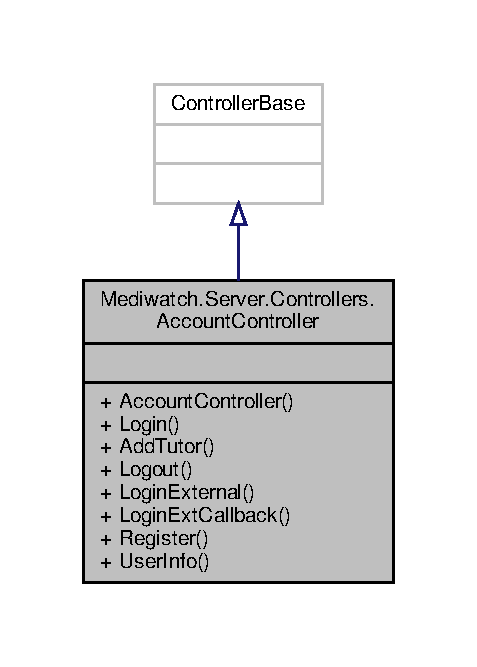
\includegraphics[width=229pt]{class_mediwatch_1_1_server_1_1_controllers_1_1_account_controller__inherit__graph}
\end{center}
\end{figure}


Graphe de collaboration de Mediwatch.\+Server.\+Controllers.\+Account\+Controller\+:\nopagebreak
\begin{figure}[H]
\begin{center}
\leavevmode
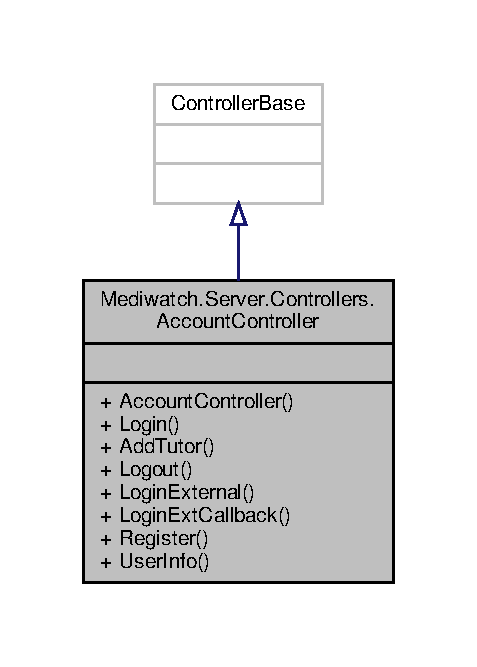
\includegraphics[width=229pt]{class_mediwatch_1_1_server_1_1_controllers_1_1_account_controller__coll__graph}
\end{center}
\end{figure}
\subsection*{Fonctions membres publiques}
\begin{DoxyCompactItemize}
\item 
\mbox{\Hypertarget{class_mediwatch_1_1_server_1_1_controllers_1_1_account_controller_ad0ec04a26c733fb1f349f7486ea820b4}\label{class_mediwatch_1_1_server_1_1_controllers_1_1_account_controller_ad0ec04a26c733fb1f349f7486ea820b4}} 
{\bfseries Account\+Controller} (Sign\+In\+Manager$<$ Identity\+User $>$ sign\+In\+Manager, User\+Manager$<$ Identity\+User $>$ user\+Manager, Role\+Manager$<$ Identity\+Role $>$ role\+Manager)
\item 
\mbox{\Hypertarget{class_mediwatch_1_1_server_1_1_controllers_1_1_account_controller_a0eca1869d875e9cdfbc6e9bc4540ae41}\label{class_mediwatch_1_1_server_1_1_controllers_1_1_account_controller_a0eca1869d875e9cdfbc6e9bc4540ae41}} 
async Task$<$ I\+Action\+Result $>$ {\bfseries Login} (Login\+Form login)
\item 
\mbox{\Hypertarget{class_mediwatch_1_1_server_1_1_controllers_1_1_account_controller_ab2521eccf3ab6c752eb5e414f6463528}\label{class_mediwatch_1_1_server_1_1_controllers_1_1_account_controller_ab2521eccf3ab6c752eb5e414f6463528}} 
async Task$<$ I\+Action\+Result $>$ {\bfseries Add\+Tutor} (string username)
\item 
\mbox{\Hypertarget{class_mediwatch_1_1_server_1_1_controllers_1_1_account_controller_a177b908ddf5a0c4ec5e3269e4cbcb252}\label{class_mediwatch_1_1_server_1_1_controllers_1_1_account_controller_a177b908ddf5a0c4ec5e3269e4cbcb252}} 
async Task$<$ I\+Action\+Result $>$ {\bfseries Logout} ()
\item 
\mbox{\Hypertarget{class_mediwatch_1_1_server_1_1_controllers_1_1_account_controller_a7f1a46f59d4b8fff4e948992fcf9f605}\label{class_mediwatch_1_1_server_1_1_controllers_1_1_account_controller_a7f1a46f59d4b8fff4e948992fcf9f605}} 
I\+Action\+Result {\bfseries Login\+External} (string hey)
\item 
\mbox{\Hypertarget{class_mediwatch_1_1_server_1_1_controllers_1_1_account_controller_ab3cb65a34f1dd5de150ebf5b956ff414}\label{class_mediwatch_1_1_server_1_1_controllers_1_1_account_controller_ab3cb65a34f1dd5de150ebf5b956ff414}} 
async Task$<$ I\+Action\+Result $>$ {\bfseries Login\+Ext\+Callback} (string return\+Url, string remote\+Error=null)
\item 
\mbox{\Hypertarget{class_mediwatch_1_1_server_1_1_controllers_1_1_account_controller_a0a0cf410c96bdacc714cb77c1d52861d}\label{class_mediwatch_1_1_server_1_1_controllers_1_1_account_controller_a0a0cf410c96bdacc714cb77c1d52861d}} 
async Task$<$ I\+Action\+Result $>$ {\bfseries Register} (Register\+Form register)
\item 
\mbox{\Hypertarget{class_mediwatch_1_1_server_1_1_controllers_1_1_account_controller_a35118ac6cb00d088863119bf4cbdc30f}\label{class_mediwatch_1_1_server_1_1_controllers_1_1_account_controller_a35118ac6cb00d088863119bf4cbdc30f}} 
User\+Information {\bfseries User\+Info} ()
\end{DoxyCompactItemize}


La documentation de cette classe a été générée à partir du fichier suivant \+:\begin{DoxyCompactItemize}
\item 
Server/\+Controllers/Account\+Controller.\+cs\end{DoxyCompactItemize}

\hypertarget{class_mediwatch_1_1_server_1_1_controllers_1_1_applicant_session_controller}{}\section{Référence de la classe Mediwatch.\+Server.\+Controllers.\+Applicant\+Session\+Controller}
\label{class_mediwatch_1_1_server_1_1_controllers_1_1_applicant_session_controller}\index{Mediwatch.\+Server.\+Controllers.\+Applicant\+Session\+Controller@{Mediwatch.\+Server.\+Controllers.\+Applicant\+Session\+Controller}}


Graphe d\textquotesingle{}héritage de Mediwatch.\+Server.\+Controllers.\+Applicant\+Session\+Controller\+:\nopagebreak
\begin{figure}[H]
\begin{center}
\leavevmode
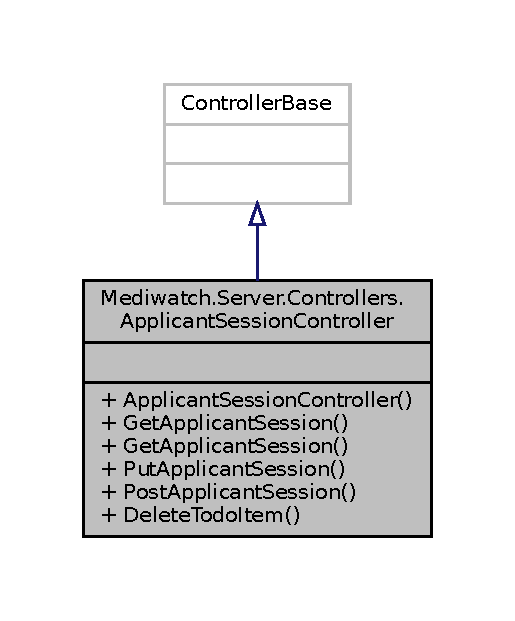
\includegraphics[width=229pt]{class_mediwatch_1_1_server_1_1_controllers_1_1_applicant_session_controller__inherit__graph}
\end{center}
\end{figure}


Graphe de collaboration de Mediwatch.\+Server.\+Controllers.\+Applicant\+Session\+Controller\+:\nopagebreak
\begin{figure}[H]
\begin{center}
\leavevmode
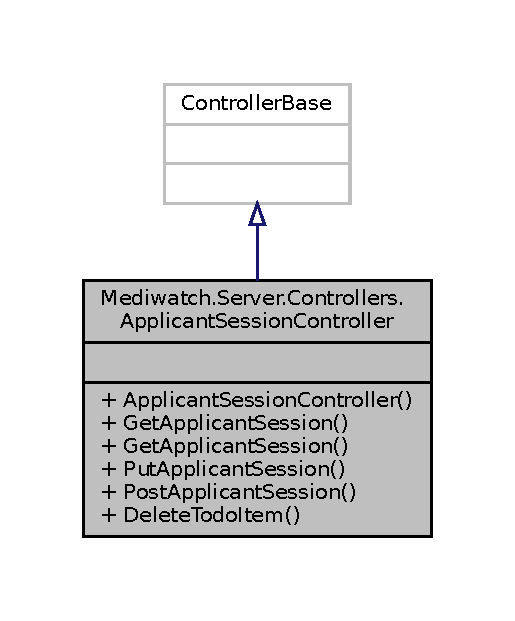
\includegraphics[width=229pt]{class_mediwatch_1_1_server_1_1_controllers_1_1_applicant_session_controller__coll__graph}
\end{center}
\end{figure}
\subsection*{Fonctions membres publiques}
\begin{DoxyCompactItemize}
\item 
\mbox{\Hypertarget{class_mediwatch_1_1_server_1_1_controllers_1_1_applicant_session_controller_a25bd4d18e93861e4d99e672b127db48b}\label{class_mediwatch_1_1_server_1_1_controllers_1_1_applicant_session_controller_a25bd4d18e93861e4d99e672b127db48b}} 
{\bfseries Applicant\+Session\+Controller} (\hyperlink{class_server_1_1_db_context_mediwatch}{Db\+Context\+Mediwatch} context)
\item 
\mbox{\Hypertarget{class_mediwatch_1_1_server_1_1_controllers_1_1_applicant_session_controller_adf8d12f5dcaaa4395522c8febae1e735}\label{class_mediwatch_1_1_server_1_1_controllers_1_1_applicant_session_controller_adf8d12f5dcaaa4395522c8febae1e735}} 
async Task$<$ Action\+Result$<$ I\+Enumerable$<$ applicant\+\_\+session $>$ $>$ $>$ {\bfseries Get\+Applicant\+Session} ()
\item 
\mbox{\Hypertarget{class_mediwatch_1_1_server_1_1_controllers_1_1_applicant_session_controller_ada65188cced0326a54f824a251869f02}\label{class_mediwatch_1_1_server_1_1_controllers_1_1_applicant_session_controller_ada65188cced0326a54f824a251869f02}} 
async Task$<$ Action\+Result$<$ applicant\+\_\+session $>$ $>$ {\bfseries Get\+Applicant\+Session} (int id)
\item 
\mbox{\Hypertarget{class_mediwatch_1_1_server_1_1_controllers_1_1_applicant_session_controller_a9b9428a2f0209f15ef65b1262e220234}\label{class_mediwatch_1_1_server_1_1_controllers_1_1_applicant_session_controller_a9b9428a2f0209f15ef65b1262e220234}} 
async Task$<$ Action\+Result$<$ applicant\+\_\+session $>$ $>$ {\bfseries Put\+Applicant\+Session} (int id, applicant\+\_\+session applicant\+Session\+Input)
\item 
\mbox{\Hypertarget{class_mediwatch_1_1_server_1_1_controllers_1_1_applicant_session_controller_a58d68c490175d8d0a13aa0104a36aed8}\label{class_mediwatch_1_1_server_1_1_controllers_1_1_applicant_session_controller_a58d68c490175d8d0a13aa0104a36aed8}} 
async Task$<$ Action\+Result$<$ applicant\+\_\+session $>$ $>$ {\bfseries Post\+Applicant\+Session} (applicant\+\_\+session applicant\+Session\+Body)
\item 
\mbox{\Hypertarget{class_mediwatch_1_1_server_1_1_controllers_1_1_applicant_session_controller_af3f0c4921fadd1483d25e39df7d5a857}\label{class_mediwatch_1_1_server_1_1_controllers_1_1_applicant_session_controller_af3f0c4921fadd1483d25e39df7d5a857}} 
async Task$<$ Action\+Result$<$ applicant\+\_\+session $>$ $>$ {\bfseries Delete\+Todo\+Item} (int id)
\end{DoxyCompactItemize}


La documentation de cette classe a été générée à partir du fichier suivant \+:\begin{DoxyCompactItemize}
\item 
Server/\+Controllers/Applicant\+Session\+Controller.\+cs\end{DoxyCompactItemize}

\hypertarget{class_blazing_blog_1_1_server_1_1_controllers_1_1_articles_controller}{}\doxysection{Référence de la classe Blazing\+Blog.\+Server.\+Controllers.\+Articles\+Controller}
\label{class_blazing_blog_1_1_server_1_1_controllers_1_1_articles_controller}\index{BlazingBlog.Server.Controllers.ArticlesController@{BlazingBlog.Server.Controllers.ArticlesController}}


Graphe d\textquotesingle{}héritage de Blazing\+Blog.\+Server.\+Controllers.\+Articles\+Controller\+:
% FIG 0


Graphe de collaboration de Blazing\+Blog.\+Server.\+Controllers.\+Articles\+Controller\+:
% FIG 1
\doxysubsection*{Fonctions membres publiques}
\begin{DoxyCompactItemize}
\item 
\mbox{\hyperlink{class_blazing_blog_1_1_server_1_1_controllers_1_1_articles_controller_a3881e802459fed1ecf975c20c9b17444}{Articles\+Controller}} (\mbox{\hyperlink{class_server_1_1_db_context_mediwatch}{Db\+Context\+Mediwatch}} context)
\item 
async Task$<$ Action\+Result$<$ I\+Enumerable$<$ Article\+Info $>$ $>$ $>$ \mbox{\hyperlink{class_blazing_blog_1_1_server_1_1_controllers_1_1_articles_controller_a9970ba338169d8ef258c10663bf211b1}{Get\+Articles\+Info}} ()
\item 
async Task$<$ Action\+Result$<$ Article $>$ $>$ \mbox{\hyperlink{class_blazing_blog_1_1_server_1_1_controllers_1_1_articles_controller_a69e1b42a4f3198d4737296e661f95a75}{Get\+Article}} (\mbox{[}From\+Query\mbox{]}string name)
\item 
async Task$<$ Action\+Result $>$ \mbox{\hyperlink{class_blazing_blog_1_1_server_1_1_controllers_1_1_articles_controller_af37d427d00f7f410f1719d8fd9a47f68}{Create\+Article}} (\mbox{[}From\+Body\mbox{]}Article article)
\end{DoxyCompactItemize}


\doxysubsection{Documentation des constructeurs et destructeur}
\mbox{\Hypertarget{class_blazing_blog_1_1_server_1_1_controllers_1_1_articles_controller_a3881e802459fed1ecf975c20c9b17444}\label{class_blazing_blog_1_1_server_1_1_controllers_1_1_articles_controller_a3881e802459fed1ecf975c20c9b17444}} 
\index{BlazingBlog.Server.Controllers.ArticlesController@{BlazingBlog.Server.Controllers.ArticlesController}!ArticlesController@{ArticlesController}}
\index{ArticlesController@{ArticlesController}!BlazingBlog.Server.Controllers.ArticlesController@{BlazingBlog.Server.Controllers.ArticlesController}}
\doxysubsubsection{\texorpdfstring{ArticlesController()}{ArticlesController()}}
{\footnotesize\ttfamily Blazing\+Blog.\+Server.\+Controllers.\+Articles\+Controller.\+Articles\+Controller (\begin{DoxyParamCaption}\item[{\mbox{\hyperlink{class_server_1_1_db_context_mediwatch}{Db\+Context\+Mediwatch}}}]{context }\end{DoxyParamCaption})}



\doxysubsection{Documentation des fonctions membres}
\mbox{\Hypertarget{class_blazing_blog_1_1_server_1_1_controllers_1_1_articles_controller_af37d427d00f7f410f1719d8fd9a47f68}\label{class_blazing_blog_1_1_server_1_1_controllers_1_1_articles_controller_af37d427d00f7f410f1719d8fd9a47f68}} 
\index{BlazingBlog.Server.Controllers.ArticlesController@{BlazingBlog.Server.Controllers.ArticlesController}!CreateArticle@{CreateArticle}}
\index{CreateArticle@{CreateArticle}!BlazingBlog.Server.Controllers.ArticlesController@{BlazingBlog.Server.Controllers.ArticlesController}}
\doxysubsubsection{\texorpdfstring{CreateArticle()}{CreateArticle()}}
{\footnotesize\ttfamily async Task$<$Action\+Result$>$ Blazing\+Blog.\+Server.\+Controllers.\+Articles\+Controller.\+Create\+Article (\begin{DoxyParamCaption}\item[{\mbox{[}\+From\+Body\mbox{]} Article}]{article }\end{DoxyParamCaption})}

\mbox{\Hypertarget{class_blazing_blog_1_1_server_1_1_controllers_1_1_articles_controller_a69e1b42a4f3198d4737296e661f95a75}\label{class_blazing_blog_1_1_server_1_1_controllers_1_1_articles_controller_a69e1b42a4f3198d4737296e661f95a75}} 
\index{BlazingBlog.Server.Controllers.ArticlesController@{BlazingBlog.Server.Controllers.ArticlesController}!GetArticle@{GetArticle}}
\index{GetArticle@{GetArticle}!BlazingBlog.Server.Controllers.ArticlesController@{BlazingBlog.Server.Controllers.ArticlesController}}
\doxysubsubsection{\texorpdfstring{GetArticle()}{GetArticle()}}
{\footnotesize\ttfamily async Task$<$Action\+Result$<$Article$>$ $>$ Blazing\+Blog.\+Server.\+Controllers.\+Articles\+Controller.\+Get\+Article (\begin{DoxyParamCaption}\item[{\mbox{[}\+From\+Query\mbox{]} string}]{name }\end{DoxyParamCaption})}

\mbox{\Hypertarget{class_blazing_blog_1_1_server_1_1_controllers_1_1_articles_controller_a9970ba338169d8ef258c10663bf211b1}\label{class_blazing_blog_1_1_server_1_1_controllers_1_1_articles_controller_a9970ba338169d8ef258c10663bf211b1}} 
\index{BlazingBlog.Server.Controllers.ArticlesController@{BlazingBlog.Server.Controllers.ArticlesController}!GetArticlesInfo@{GetArticlesInfo}}
\index{GetArticlesInfo@{GetArticlesInfo}!BlazingBlog.Server.Controllers.ArticlesController@{BlazingBlog.Server.Controllers.ArticlesController}}
\doxysubsubsection{\texorpdfstring{GetArticlesInfo()}{GetArticlesInfo()}}
{\footnotesize\ttfamily async Task$<$Action\+Result$<$I\+Enumerable$<$Article\+Info$>$ $>$ $>$ Blazing\+Blog.\+Server.\+Controllers.\+Articles\+Controller.\+Get\+Articles\+Info (\begin{DoxyParamCaption}{ }\end{DoxyParamCaption})}



La documentation de cette classe a été générée à partir du fichier suivant \+:\begin{DoxyCompactItemize}
\item 
Server/\+Controllers/\mbox{\hyperlink{_articles_controller_8cs}{Articles\+Controller.\+cs}}\end{DoxyCompactItemize}

\hypertarget{class_blazing_blog_1_1_server_1_1_controllers_1_1_blog_utils_controller}{}\doxysection{Référence de la classe Blazing\+Blog.\+Server.\+Controllers.\+Blog\+Utils\+Controller}
\label{class_blazing_blog_1_1_server_1_1_controllers_1_1_blog_utils_controller}\index{BlazingBlog.Server.Controllers.BlogUtilsController@{BlazingBlog.Server.Controllers.BlogUtilsController}}


Graphe d\textquotesingle{}héritage de Blazing\+Blog.\+Server.\+Controllers.\+Blog\+Utils\+Controller\+:\nopagebreak
\begin{figure}[H]
\begin{center}
\leavevmode
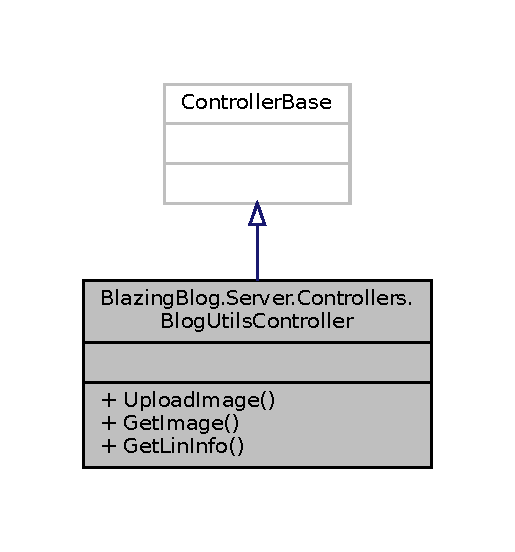
\includegraphics[width=247pt]{class_blazing_blog_1_1_server_1_1_controllers_1_1_blog_utils_controller__inherit__graph}
\end{center}
\end{figure}


Graphe de collaboration de Blazing\+Blog.\+Server.\+Controllers.\+Blog\+Utils\+Controller\+:\nopagebreak
\begin{figure}[H]
\begin{center}
\leavevmode
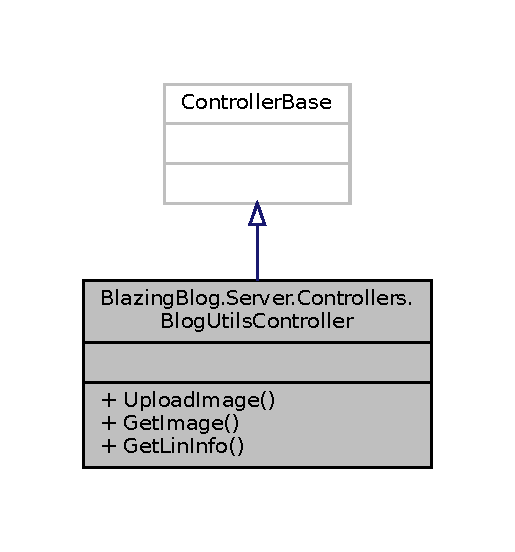
\includegraphics[width=247pt]{class_blazing_blog_1_1_server_1_1_controllers_1_1_blog_utils_controller__coll__graph}
\end{center}
\end{figure}
\doxysubsection*{Fonctions membres publiques}
\begin{DoxyCompactItemize}
\item 
async Task$<$ \mbox{\hyperlink{class_blazing_blog_1_1_shared_1_1_image_upload}{Image\+Upload}} $>$ \mbox{\hyperlink{class_blazing_blog_1_1_server_1_1_controllers_1_1_blog_utils_controller_a7e2fd0bf2bf61c62ad1598d787987776}{Upload\+Image}} ()
\begin{DoxyCompactList}\small\item\em A\+PI P\+O\+ST\+: /\+Blog\+Utils/\+Upload\+Image Upload Image to the server \end{DoxyCompactList}\item 
I\+Action\+Result \mbox{\hyperlink{class_blazing_blog_1_1_server_1_1_controllers_1_1_blog_utils_controller_abd681dd8b9f613ebca29900f87c763b9}{Get\+Image}} (\mbox{[}From\+Query\mbox{]} string file\+Name, \mbox{[}From\+Query\mbox{]} string content\+Type)
\begin{DoxyCompactList}\small\item\em Get Image from image uploaded on the server G\+ET\+: /\+Blog\+Utils/\+Get\+Image \end{DoxyCompactList}\item 
\mbox{\hyperlink{class_blazing_blog_1_1_shared_1_1_link_description}{Link\+Description}} \mbox{\hyperlink{class_blazing_blog_1_1_server_1_1_controllers_1_1_blog_utils_controller_abb07a81ee10a101acbc979c4a217a76a}{Get\+Lin\+Info}} (string url)
\begin{DoxyCompactList}\small\item\em G\+ET\+: /\+Blog\+Utils/\+Get\+Lin\+Info Give link info for preview \end{DoxyCompactList}\end{DoxyCompactItemize}


\doxysubsection{Documentation des fonctions membres}
\mbox{\Hypertarget{class_blazing_blog_1_1_server_1_1_controllers_1_1_blog_utils_controller_abd681dd8b9f613ebca29900f87c763b9}\label{class_blazing_blog_1_1_server_1_1_controllers_1_1_blog_utils_controller_abd681dd8b9f613ebca29900f87c763b9}} 
\index{BlazingBlog.Server.Controllers.BlogUtilsController@{BlazingBlog.Server.Controllers.BlogUtilsController}!GetImage@{GetImage}}
\index{GetImage@{GetImage}!BlazingBlog.Server.Controllers.BlogUtilsController@{BlazingBlog.Server.Controllers.BlogUtilsController}}
\doxysubsubsection{\texorpdfstring{GetImage()}{GetImage()}}
{\footnotesize\ttfamily I\+Action\+Result Blazing\+Blog.\+Server.\+Controllers.\+Blog\+Utils\+Controller.\+Get\+Image (\begin{DoxyParamCaption}\item[{\mbox{[}\+From\+Query\mbox{]} string}]{file\+Name,  }\item[{\mbox{[}\+From\+Query\mbox{]} string}]{content\+Type }\end{DoxyParamCaption})\hspace{0.3cm}{\ttfamily [inline]}}



Get Image from image uploaded on the server G\+ET\+: /\+Blog\+Utils/\+Get\+Image 


\begin{DoxyParams}{Paramètres}
{\em file\+Name} & the path from the folder which the images are stocked\\
\hline
{\em content\+Type} & the type of image to get\\
\hline
\end{DoxyParams}
\begin{DoxyReturn}{Renvoie}
the Image in raw
\end{DoxyReturn}
\mbox{\Hypertarget{class_blazing_blog_1_1_server_1_1_controllers_1_1_blog_utils_controller_abb07a81ee10a101acbc979c4a217a76a}\label{class_blazing_blog_1_1_server_1_1_controllers_1_1_blog_utils_controller_abb07a81ee10a101acbc979c4a217a76a}} 
\index{BlazingBlog.Server.Controllers.BlogUtilsController@{BlazingBlog.Server.Controllers.BlogUtilsController}!GetLinInfo@{GetLinInfo}}
\index{GetLinInfo@{GetLinInfo}!BlazingBlog.Server.Controllers.BlogUtilsController@{BlazingBlog.Server.Controllers.BlogUtilsController}}
\doxysubsubsection{\texorpdfstring{GetLinInfo()}{GetLinInfo()}}
{\footnotesize\ttfamily \mbox{\hyperlink{class_blazing_blog_1_1_shared_1_1_link_description}{Link\+Description}} Blazing\+Blog.\+Server.\+Controllers.\+Blog\+Utils\+Controller.\+Get\+Lin\+Info (\begin{DoxyParamCaption}\item[{string}]{url }\end{DoxyParamCaption})\hspace{0.3cm}{\ttfamily [inline]}}



G\+ET\+: /\+Blog\+Utils/\+Get\+Lin\+Info Give link info for preview 


\begin{DoxyParams}{Paramètres}
{\em url} & Url\\
\hline
\end{DoxyParams}
\begin{DoxyReturn}{Renvoie}
a link descrition base on the url
\end{DoxyReturn}
\mbox{\Hypertarget{class_blazing_blog_1_1_server_1_1_controllers_1_1_blog_utils_controller_a7e2fd0bf2bf61c62ad1598d787987776}\label{class_blazing_blog_1_1_server_1_1_controllers_1_1_blog_utils_controller_a7e2fd0bf2bf61c62ad1598d787987776}} 
\index{BlazingBlog.Server.Controllers.BlogUtilsController@{BlazingBlog.Server.Controllers.BlogUtilsController}!UploadImage@{UploadImage}}
\index{UploadImage@{UploadImage}!BlazingBlog.Server.Controllers.BlogUtilsController@{BlazingBlog.Server.Controllers.BlogUtilsController}}
\doxysubsubsection{\texorpdfstring{UploadImage()}{UploadImage()}}
{\footnotesize\ttfamily async Task$<$\mbox{\hyperlink{class_blazing_blog_1_1_shared_1_1_image_upload}{Image\+Upload}}$>$ Blazing\+Blog.\+Server.\+Controllers.\+Blog\+Utils\+Controller.\+Upload\+Image (\begin{DoxyParamCaption}{ }\end{DoxyParamCaption})\hspace{0.3cm}{\ttfamily [inline]}}



A\+PI P\+O\+ST\+: /\+Blog\+Utils/\+Upload\+Image Upload Image to the server 

\begin{DoxyReturn}{Renvoie}
return the image informations
\end{DoxyReturn}


La documentation de cette classe a été générée à partir du fichier suivant \+:\begin{DoxyCompactItemize}
\item 
Server/\+Controllers/Blog\+Utils\+Controller.\+cs\end{DoxyCompactItemize}

\hypertarget{class_mediwatch_1_1_server_1_1_controllers_1_1_compagny_controller}{}\doxysection{Référence de la classe Mediwatch.\+Server.\+Controllers.\+Compagny\+Controller}
\label{class_mediwatch_1_1_server_1_1_controllers_1_1_compagny_controller}\index{Mediwatch.Server.Controllers.CompagnyController@{Mediwatch.Server.Controllers.CompagnyController}}


Graphe d\textquotesingle{}héritage de Mediwatch.\+Server.\+Controllers.\+Compagny\+Controller\+:
\nopagebreak
\begin{figure}[H]
\begin{center}
\leavevmode
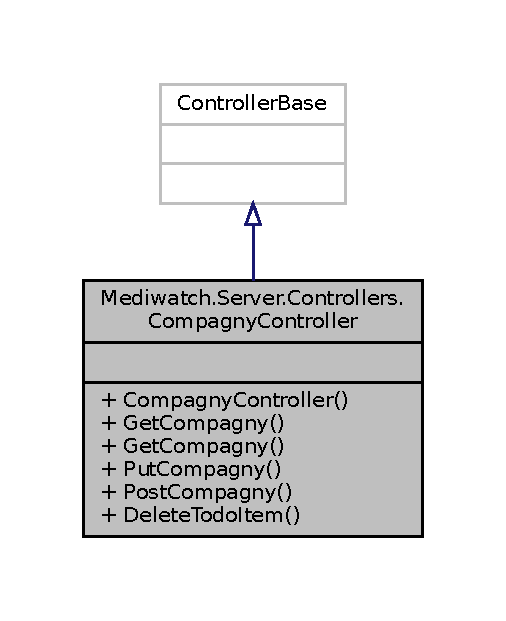
\includegraphics[width=243pt]{class_mediwatch_1_1_server_1_1_controllers_1_1_compagny_controller__inherit__graph}
\end{center}
\end{figure}


Graphe de collaboration de Mediwatch.\+Server.\+Controllers.\+Compagny\+Controller\+:
\nopagebreak
\begin{figure}[H]
\begin{center}
\leavevmode
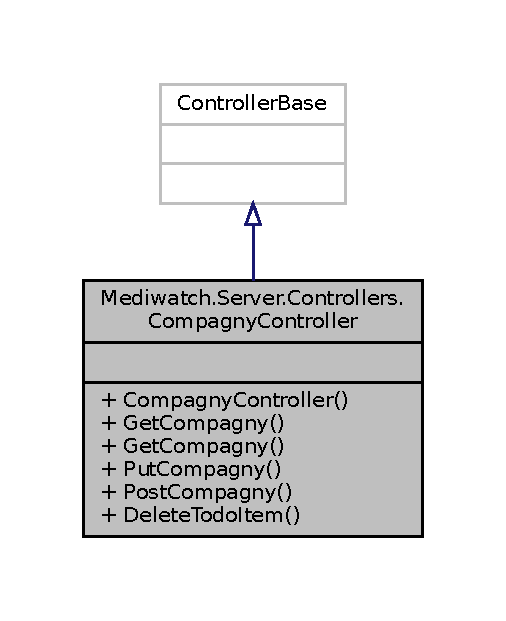
\includegraphics[width=243pt]{class_mediwatch_1_1_server_1_1_controllers_1_1_compagny_controller__coll__graph}
\end{center}
\end{figure}
\doxysubsection*{Fonctions membres publiques}
\begin{DoxyCompactItemize}
\item 
\mbox{\Hypertarget{class_mediwatch_1_1_server_1_1_controllers_1_1_compagny_controller_ab4a8837fdb737884b3248ee77f734ad0}\label{class_mediwatch_1_1_server_1_1_controllers_1_1_compagny_controller_ab4a8837fdb737884b3248ee77f734ad0}} 
{\bfseries Compagny\+Controller} (\mbox{\hyperlink{class_server_1_1_db_context_mediwatch}{Db\+Context\+Mediwatch}} context)
\item 
async Task$<$ Action\+Result$<$ I\+Enumerable$<$ compagny $>$ $>$ $>$ \mbox{\hyperlink{class_mediwatch_1_1_server_1_1_controllers_1_1_compagny_controller_a7bc69ceda49f9017a2d6ddfdbffe4758}{Get\+Compagny}} ()
\item 
async Task$<$ Action\+Result$<$ compagny $>$ $>$ \mbox{\hyperlink{class_mediwatch_1_1_server_1_1_controllers_1_1_compagny_controller_a6608c7128f9e7b31b04885ef1d7e004d}{Get\+Compagny}} (int id)
\item 
async Task$<$ Action\+Result$<$ compagny $>$ $>$ \mbox{\hyperlink{class_mediwatch_1_1_server_1_1_controllers_1_1_compagny_controller_a6d092dd8d9edcd60e4a38e1d90af3e40}{Put\+Compagny}} (int id, compagny compagny\+Input)
\item 
async Task$<$ Action\+Result$<$ compagny $>$ $>$ \mbox{\hyperlink{class_mediwatch_1_1_server_1_1_controllers_1_1_compagny_controller_ad144f627b336f3e43ba994fbdd9c9419}{Post\+Compagny}} (compagny compagny\+Body)
\item 
async Task$<$ Action\+Result$<$ compagny $>$ $>$ \mbox{\hyperlink{class_mediwatch_1_1_server_1_1_controllers_1_1_compagny_controller_a5c33b6687ecca9c5b060f029ce809e7d}{Delete\+Todo\+Item}} (int id)
\end{DoxyCompactItemize}


\doxysubsection{Documentation des fonctions membres}
\mbox{\Hypertarget{class_mediwatch_1_1_server_1_1_controllers_1_1_compagny_controller_a5c33b6687ecca9c5b060f029ce809e7d}\label{class_mediwatch_1_1_server_1_1_controllers_1_1_compagny_controller_a5c33b6687ecca9c5b060f029ce809e7d}} 
\index{Mediwatch.Server.Controllers.CompagnyController@{Mediwatch.Server.Controllers.CompagnyController}!DeleteTodoItem@{DeleteTodoItem}}
\index{DeleteTodoItem@{DeleteTodoItem}!Mediwatch.Server.Controllers.CompagnyController@{Mediwatch.Server.Controllers.CompagnyController}}
\doxysubsubsection{\texorpdfstring{DeleteTodoItem()}{DeleteTodoItem()}}
{\footnotesize\ttfamily async Task$<$Action\+Result$<$compagny$>$ $>$ Mediwatch.\+Server.\+Controllers.\+Compagny\+Controller.\+Delete\+Todo\+Item (\begin{DoxyParamCaption}\item[{int}]{id }\end{DoxyParamCaption})\hspace{0.3cm}{\ttfamily [inline]}}

Delete the company ID 

\begin{DoxyReturn}{Renvoie}

\end{DoxyReturn}
\mbox{\Hypertarget{class_mediwatch_1_1_server_1_1_controllers_1_1_compagny_controller_a7bc69ceda49f9017a2d6ddfdbffe4758}\label{class_mediwatch_1_1_server_1_1_controllers_1_1_compagny_controller_a7bc69ceda49f9017a2d6ddfdbffe4758}} 
\index{Mediwatch.Server.Controllers.CompagnyController@{Mediwatch.Server.Controllers.CompagnyController}!GetCompagny@{GetCompagny}}
\index{GetCompagny@{GetCompagny}!Mediwatch.Server.Controllers.CompagnyController@{Mediwatch.Server.Controllers.CompagnyController}}
\doxysubsubsection{\texorpdfstring{GetCompagny()}{GetCompagny()}\hspace{0.1cm}{\footnotesize\ttfamily [1/2]}}
{\footnotesize\ttfamily async Task$<$Action\+Result$<$I\+Enumerable$<$compagny$>$ $>$ $>$ Mediwatch.\+Server.\+Controllers.\+Compagny\+Controller.\+Get\+Compagny (\begin{DoxyParamCaption}{ }\end{DoxyParamCaption})\hspace{0.3cm}{\ttfamily [inline]}}

Get all compagny 

\begin{DoxyReturn}{Renvoie}
Json raw list of compgny
\end{DoxyReturn}
\mbox{\Hypertarget{class_mediwatch_1_1_server_1_1_controllers_1_1_compagny_controller_a6608c7128f9e7b31b04885ef1d7e004d}\label{class_mediwatch_1_1_server_1_1_controllers_1_1_compagny_controller_a6608c7128f9e7b31b04885ef1d7e004d}} 
\index{Mediwatch.Server.Controllers.CompagnyController@{Mediwatch.Server.Controllers.CompagnyController}!GetCompagny@{GetCompagny}}
\index{GetCompagny@{GetCompagny}!Mediwatch.Server.Controllers.CompagnyController@{Mediwatch.Server.Controllers.CompagnyController}}
\doxysubsubsection{\texorpdfstring{GetCompagny()}{GetCompagny()}\hspace{0.1cm}{\footnotesize\ttfamily [2/2]}}
{\footnotesize\ttfamily async Task$<$Action\+Result$<$compagny$>$ $>$ Mediwatch.\+Server.\+Controllers.\+Compagny\+Controller.\+Get\+Compagny (\begin{DoxyParamCaption}\item[{int}]{id }\end{DoxyParamCaption})\hspace{0.3cm}{\ttfamily [inline]}}

Get a compagny by its id 

\begin{DoxyReturn}{Renvoie}
Return the company data
\end{DoxyReturn}
\mbox{\Hypertarget{class_mediwatch_1_1_server_1_1_controllers_1_1_compagny_controller_ad144f627b336f3e43ba994fbdd9c9419}\label{class_mediwatch_1_1_server_1_1_controllers_1_1_compagny_controller_ad144f627b336f3e43ba994fbdd9c9419}} 
\index{Mediwatch.Server.Controllers.CompagnyController@{Mediwatch.Server.Controllers.CompagnyController}!PostCompagny@{PostCompagny}}
\index{PostCompagny@{PostCompagny}!Mediwatch.Server.Controllers.CompagnyController@{Mediwatch.Server.Controllers.CompagnyController}}
\doxysubsubsection{\texorpdfstring{PostCompagny()}{PostCompagny()}}
{\footnotesize\ttfamily async Task$<$Action\+Result$<$compagny$>$ $>$ Mediwatch.\+Server.\+Controllers.\+Compagny\+Controller.\+Post\+Compagny (\begin{DoxyParamCaption}\item[{compagny}]{compagny\+Body }\end{DoxyParamCaption})\hspace{0.3cm}{\ttfamily [inline]}}

Create a new compagny \mbox{\Hypertarget{class_mediwatch_1_1_server_1_1_controllers_1_1_compagny_controller_a6d092dd8d9edcd60e4a38e1d90af3e40}\label{class_mediwatch_1_1_server_1_1_controllers_1_1_compagny_controller_a6d092dd8d9edcd60e4a38e1d90af3e40}} 
\index{Mediwatch.Server.Controllers.CompagnyController@{Mediwatch.Server.Controllers.CompagnyController}!PutCompagny@{PutCompagny}}
\index{PutCompagny@{PutCompagny}!Mediwatch.Server.Controllers.CompagnyController@{Mediwatch.Server.Controllers.CompagnyController}}
\doxysubsubsection{\texorpdfstring{PutCompagny()}{PutCompagny()}}
{\footnotesize\ttfamily async Task$<$Action\+Result$<$compagny$>$ $>$ Mediwatch.\+Server.\+Controllers.\+Compagny\+Controller.\+Put\+Compagny (\begin{DoxyParamCaption}\item[{int}]{id,  }\item[{compagny}]{compagny\+Input }\end{DoxyParamCaption})\hspace{0.3cm}{\ttfamily [inline]}}

Edit the compagny information specified by its id 

~\newline


La documentation de cette classe a été générée à partir du fichier suivant \+:\begin{DoxyCompactItemize}
\item 
Server/\+Controllers/Compagny\+Controller.\+cs\end{DoxyCompactItemize}

\hypertarget{class_server_1_1_db_context_mediwatch}{}\doxysection{Référence de la classe Server.\+Db\+Context\+Mediwatch}
\label{class_server_1_1_db_context_mediwatch}\index{Server.DbContextMediwatch@{Server.DbContextMediwatch}}


Graphe d\textquotesingle{}héritage de Server.\+Db\+Context\+Mediwatch\+:
\nopagebreak
\begin{figure}[H]
\begin{center}
\leavevmode
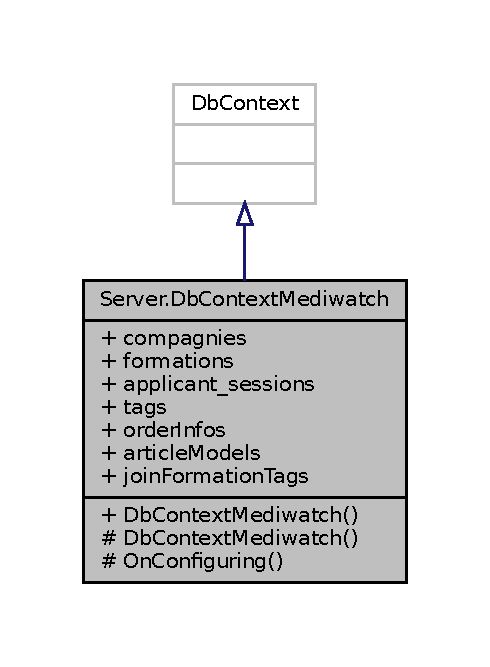
\includegraphics[width=235pt]{class_server_1_1_db_context_mediwatch__inherit__graph}
\end{center}
\end{figure}


Graphe de collaboration de Server.\+Db\+Context\+Mediwatch\+:
\nopagebreak
\begin{figure}[H]
\begin{center}
\leavevmode
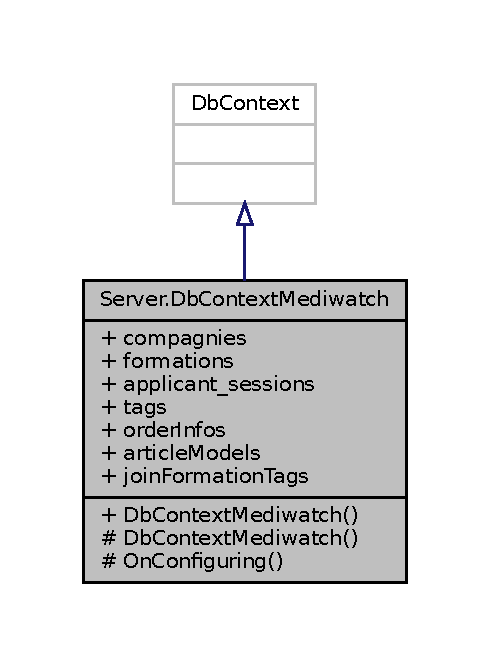
\includegraphics[width=235pt]{class_server_1_1_db_context_mediwatch__coll__graph}
\end{center}
\end{figure}
\doxysubsection*{Fonctions membres publiques}
\begin{DoxyCompactItemize}
\item 
\mbox{\Hypertarget{class_server_1_1_db_context_mediwatch_a94fde86883fe0a2d1ce0b4c58f06727f}\label{class_server_1_1_db_context_mediwatch_a94fde86883fe0a2d1ce0b4c58f06727f}} 
{\bfseries Db\+Context\+Mediwatch} (Db\+Context\+Options$<$ \mbox{\hyperlink{class_server_1_1_db_context_mediwatch}{Db\+Context\+Mediwatch}} $>$ options)
\end{DoxyCompactItemize}
\doxysubsection*{Fonctions membres protégées}
\begin{DoxyCompactItemize}
\item 
\mbox{\Hypertarget{class_server_1_1_db_context_mediwatch_a72073ff88f3990c4792f85688f55f073}\label{class_server_1_1_db_context_mediwatch_a72073ff88f3990c4792f85688f55f073}} 
override void {\bfseries On\+Configuring} (Db\+Context\+Options\+Builder options)
\end{DoxyCompactItemize}
\doxysubsection*{Propriétés}
\begin{DoxyCompactItemize}
\item 
\mbox{\Hypertarget{class_server_1_1_db_context_mediwatch_a068d9222b8448c069c2d181a9f577d0c}\label{class_server_1_1_db_context_mediwatch_a068d9222b8448c069c2d181a9f577d0c}} 
Db\+Set$<$ compagny $>$ {\bfseries compagnies}\hspace{0.3cm}{\ttfamily  \mbox{[}get, set\mbox{]}}
\item 
\mbox{\Hypertarget{class_server_1_1_db_context_mediwatch_a6597dab2848cd5aa87774af4bf6eb4e4}\label{class_server_1_1_db_context_mediwatch_a6597dab2848cd5aa87774af4bf6eb4e4}} 
Db\+Set$<$ formation $>$ {\bfseries formations}\hspace{0.3cm}{\ttfamily  \mbox{[}get, set\mbox{]}}
\item 
\mbox{\Hypertarget{class_server_1_1_db_context_mediwatch_aea8aaf9d1c1f27f64a2a488f41c531b2}\label{class_server_1_1_db_context_mediwatch_aea8aaf9d1c1f27f64a2a488f41c531b2}} 
Db\+Set$<$ applicant\+\_\+session $>$ {\bfseries applicant\+\_\+sessions}\hspace{0.3cm}{\ttfamily  \mbox{[}get, set\mbox{]}}
\item 
\mbox{\Hypertarget{class_server_1_1_db_context_mediwatch_a0bcaba8827c3d82857deb35923f6dcef}\label{class_server_1_1_db_context_mediwatch_a0bcaba8827c3d82857deb35923f6dcef}} 
Db\+Set$<$ tag $>$ {\bfseries tags}\hspace{0.3cm}{\ttfamily  \mbox{[}get, set\mbox{]}}
\item 
\mbox{\Hypertarget{class_server_1_1_db_context_mediwatch_a852541740bc368d71f6816d4e4c3be86}\label{class_server_1_1_db_context_mediwatch_a852541740bc368d71f6816d4e4c3be86}} 
Db\+Set$<$ order\+Info $>$ {\bfseries order\+Infos}\hspace{0.3cm}{\ttfamily  \mbox{[}get, set\mbox{]}}
\item 
\mbox{\Hypertarget{class_server_1_1_db_context_mediwatch_a298accc740bb1638718fe4664b41e800}\label{class_server_1_1_db_context_mediwatch_a298accc740bb1638718fe4664b41e800}} 
Db\+Set$<$ Blazing\+Article\+Model $>$ {\bfseries article\+Models}\hspace{0.3cm}{\ttfamily  \mbox{[}get, set\mbox{]}}
\end{DoxyCompactItemize}


La documentation de cette classe a été générée à partir du fichier suivant \+:\begin{DoxyCompactItemize}
\item 
Server/Db\+Context\+Mediwatch.\+cs\end{DoxyCompactItemize}

\hypertarget{class_mediwatch_1_1_server_1_1_migrations_1_1_db_context_mediwatch_model_snapshot}{}\section{Référence de la classe Mediwatch.\+Server.\+Migrations.\+Db\+Context\+Mediwatch\+Model\+Snapshot}
\label{class_mediwatch_1_1_server_1_1_migrations_1_1_db_context_mediwatch_model_snapshot}\index{Mediwatch.\+Server.\+Migrations.\+Db\+Context\+Mediwatch\+Model\+Snapshot@{Mediwatch.\+Server.\+Migrations.\+Db\+Context\+Mediwatch\+Model\+Snapshot}}


Graphe d\textquotesingle{}héritage de Mediwatch.\+Server.\+Migrations.\+Db\+Context\+Mediwatch\+Model\+Snapshot\+:\nopagebreak
\begin{figure}[H]
\begin{center}
\leavevmode
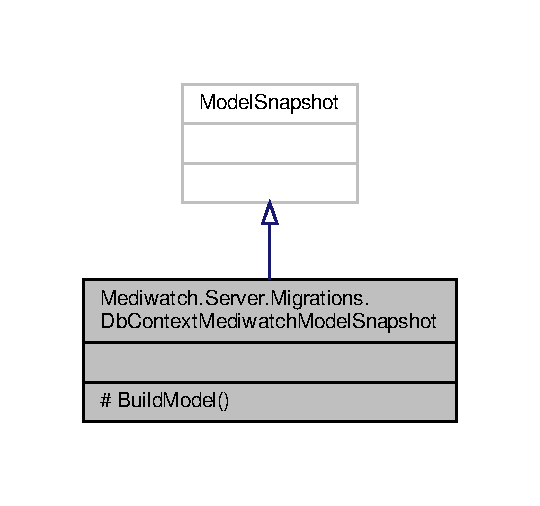
\includegraphics[width=259pt]{class_mediwatch_1_1_server_1_1_migrations_1_1_db_context_mediwatch_model_snapshot__inherit__graph}
\end{center}
\end{figure}


Graphe de collaboration de Mediwatch.\+Server.\+Migrations.\+Db\+Context\+Mediwatch\+Model\+Snapshot\+:\nopagebreak
\begin{figure}[H]
\begin{center}
\leavevmode
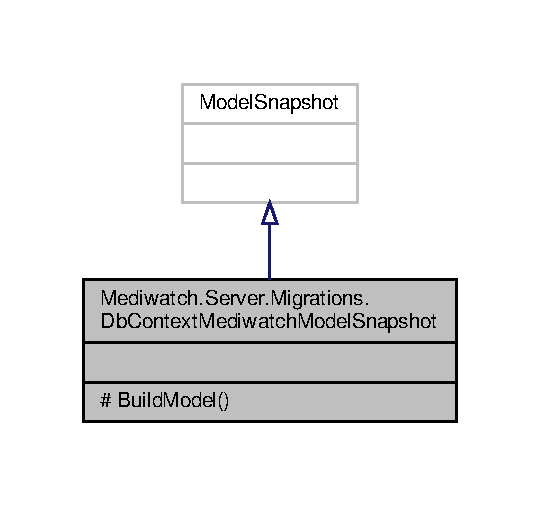
\includegraphics[width=259pt]{class_mediwatch_1_1_server_1_1_migrations_1_1_db_context_mediwatch_model_snapshot__coll__graph}
\end{center}
\end{figure}
\subsection*{Fonctions membres protégées}
\begin{DoxyCompactItemize}
\item 
\mbox{\Hypertarget{class_mediwatch_1_1_server_1_1_migrations_1_1_db_context_mediwatch_model_snapshot_a2b90b9a1956a9ceb7f881aa62d6c8ac3}\label{class_mediwatch_1_1_server_1_1_migrations_1_1_db_context_mediwatch_model_snapshot_a2b90b9a1956a9ceb7f881aa62d6c8ac3}} 
override void {\bfseries Build\+Model} (Model\+Builder model\+Builder)
\end{DoxyCompactItemize}


La documentation de cette classe a été générée à partir du fichier suivant \+:\begin{DoxyCompactItemize}
\item 
Server/\+Migrations/Db\+Context\+Mediwatch\+Model\+Snapshot.\+cs\end{DoxyCompactItemize}

\hypertarget{class_mediwatch_1_1_server_1_1_pages_1_1_error_model}{}\doxysection{Référence de la classe Mediwatch.\+Server.\+Pages.\+Error\+Model}
\label{class_mediwatch_1_1_server_1_1_pages_1_1_error_model}\index{Mediwatch.Server.Pages.ErrorModel@{Mediwatch.Server.Pages.ErrorModel}}


Graphe d\textquotesingle{}héritage de Mediwatch.\+Server.\+Pages.\+Error\+Model\+:\nopagebreak
\begin{figure}[H]
\begin{center}
\leavevmode
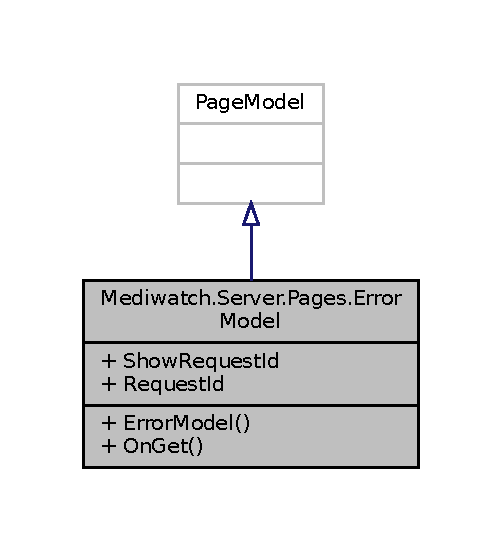
\includegraphics[width=241pt]{class_mediwatch_1_1_server_1_1_pages_1_1_error_model__inherit__graph}
\end{center}
\end{figure}


Graphe de collaboration de Mediwatch.\+Server.\+Pages.\+Error\+Model\+:\nopagebreak
\begin{figure}[H]
\begin{center}
\leavevmode
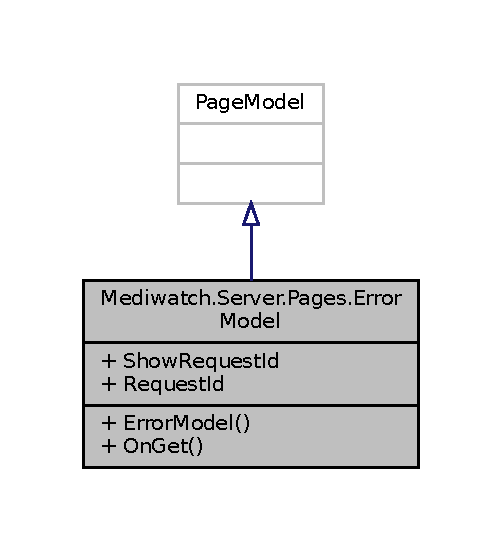
\includegraphics[width=241pt]{class_mediwatch_1_1_server_1_1_pages_1_1_error_model__coll__graph}
\end{center}
\end{figure}
\doxysubsection*{Fonctions membres publiques}
\begin{DoxyCompactItemize}
\item 
\mbox{\Hypertarget{class_mediwatch_1_1_server_1_1_pages_1_1_error_model_a6071f8072c63f30c32dac09a811f9ab3}\label{class_mediwatch_1_1_server_1_1_pages_1_1_error_model_a6071f8072c63f30c32dac09a811f9ab3}} 
{\bfseries Error\+Model} (I\+Logger$<$ \mbox{\hyperlink{class_mediwatch_1_1_server_1_1_pages_1_1_error_model}{Error\+Model}} $>$ logger)
\item 
\mbox{\Hypertarget{class_mediwatch_1_1_server_1_1_pages_1_1_error_model_afff141d7facfcb25a4a05e433cb18369}\label{class_mediwatch_1_1_server_1_1_pages_1_1_error_model_afff141d7facfcb25a4a05e433cb18369}} 
void {\bfseries On\+Get} ()
\end{DoxyCompactItemize}
\doxysubsection*{Attributs publics}
\begin{DoxyCompactItemize}
\item 
\mbox{\Hypertarget{class_mediwatch_1_1_server_1_1_pages_1_1_error_model_a63bd289fd620d1418adcd60cc4ff7f53}\label{class_mediwatch_1_1_server_1_1_pages_1_1_error_model_a63bd289fd620d1418adcd60cc4ff7f53}} 
bool {\bfseries Show\+Request\+Id} =$>$ !string.\+Is\+Null\+Or\+Empty(Request\+Id)
\end{DoxyCompactItemize}
\doxysubsection*{Propriétés}
\begin{DoxyCompactItemize}
\item 
\mbox{\Hypertarget{class_mediwatch_1_1_server_1_1_pages_1_1_error_model_a6b1ab7a6328fa0b58ac9b76c0d8bfbef}\label{class_mediwatch_1_1_server_1_1_pages_1_1_error_model_a6b1ab7a6328fa0b58ac9b76c0d8bfbef}} 
string {\bfseries Request\+Id}\hspace{0.3cm}{\ttfamily  \mbox{[}get, set\mbox{]}}
\end{DoxyCompactItemize}


La documentation de cette classe a été générée à partir du fichier suivant \+:\begin{DoxyCompactItemize}
\item 
Server/\+Pages/Error.\+cshtml.\+cs\end{DoxyCompactItemize}

\hypertarget{class_mediwatch_1_1_server_1_1_controllers_1_1_formation_controller}{}\doxysection{Référence de la classe Mediwatch.\+Server.\+Controllers.\+Formation\+Controller}
\label{class_mediwatch_1_1_server_1_1_controllers_1_1_formation_controller}\index{Mediwatch.Server.Controllers.FormationController@{Mediwatch.Server.Controllers.FormationController}}


Graphe d\textquotesingle{}héritage de Mediwatch.\+Server.\+Controllers.\+Formation\+Controller\+:
\nopagebreak
\begin{figure}[H]
\begin{center}
\leavevmode
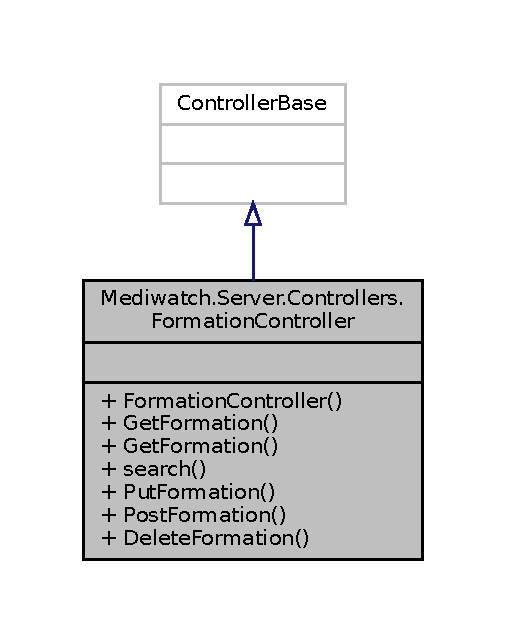
\includegraphics[width=243pt]{class_mediwatch_1_1_server_1_1_controllers_1_1_formation_controller__inherit__graph}
\end{center}
\end{figure}


Graphe de collaboration de Mediwatch.\+Server.\+Controllers.\+Formation\+Controller\+:
\nopagebreak
\begin{figure}[H]
\begin{center}
\leavevmode
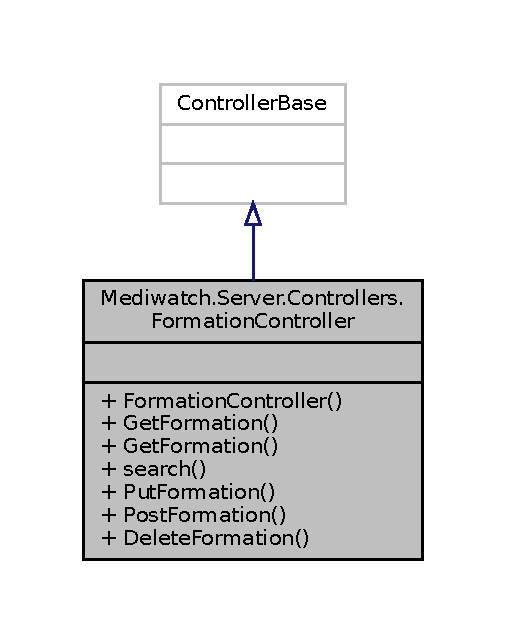
\includegraphics[width=243pt]{class_mediwatch_1_1_server_1_1_controllers_1_1_formation_controller__coll__graph}
\end{center}
\end{figure}
\doxysubsection*{Fonctions membres publiques}
\begin{DoxyCompactItemize}
\item 
\mbox{\Hypertarget{class_mediwatch_1_1_server_1_1_controllers_1_1_formation_controller_a71430327b82736d6b252d83a40833dbd}\label{class_mediwatch_1_1_server_1_1_controllers_1_1_formation_controller_a71430327b82736d6b252d83a40833dbd}} 
{\bfseries Formation\+Controller} (\mbox{\hyperlink{class_server_1_1_db_context_mediwatch}{Db\+Context\+Mediwatch}} context)
\item 
async Task$<$ Action\+Result$<$ I\+Enumerable$<$ formation $>$ $>$ $>$ \mbox{\hyperlink{class_mediwatch_1_1_server_1_1_controllers_1_1_formation_controller_ac1711d7a1c8bbd44715fc57cb945c93c}{Get\+Formation}} ()
\item 
async Task$<$ Action\+Result$<$ formation $>$ $>$ \mbox{\hyperlink{class_mediwatch_1_1_server_1_1_controllers_1_1_formation_controller_aecf887fc57ba8ee1af0ba1be7703738a}{Get\+Formation}} (int id)
\item 
async Task$<$ Action\+Result$<$ formation $>$ $>$ \mbox{\hyperlink{class_mediwatch_1_1_server_1_1_controllers_1_1_formation_controller_ac56853c9a6cf3b7cb2303d1c6bf8a037}{Put\+Formation}} (int id, formation formation\+Put)
\item 
async Task$<$ Action\+Result$<$ formation $>$ $>$ \mbox{\hyperlink{class_mediwatch_1_1_server_1_1_controllers_1_1_formation_controller_a2710e701c2d495ee6a1d343a5303bfa3}{Post\+Formation}} (formation formation\+Body)
\item 
async Task$<$ Action\+Result$<$ formation $>$ $>$ \mbox{\hyperlink{class_mediwatch_1_1_server_1_1_controllers_1_1_formation_controller_af3e300009a2f7d0d1551da387effbe09}{Delete\+Formation}} (int id)
\end{DoxyCompactItemize}


\doxysubsection{Documentation des fonctions membres}
\mbox{\Hypertarget{class_mediwatch_1_1_server_1_1_controllers_1_1_formation_controller_af3e300009a2f7d0d1551da387effbe09}\label{class_mediwatch_1_1_server_1_1_controllers_1_1_formation_controller_af3e300009a2f7d0d1551da387effbe09}} 
\index{Mediwatch.Server.Controllers.FormationController@{Mediwatch.Server.Controllers.FormationController}!DeleteFormation@{DeleteFormation}}
\index{DeleteFormation@{DeleteFormation}!Mediwatch.Server.Controllers.FormationController@{Mediwatch.Server.Controllers.FormationController}}
\doxysubsubsection{\texorpdfstring{DeleteFormation()}{DeleteFormation()}}
{\footnotesize\ttfamily async Task$<$Action\+Result$<$formation$>$ $>$ Mediwatch.\+Server.\+Controllers.\+Formation\+Controller.\+Delete\+Formation (\begin{DoxyParamCaption}\item[{int}]{id }\end{DoxyParamCaption})\hspace{0.3cm}{\ttfamily [inline]}}

Delete the formation by ID 

\begin{DoxyReturn}{Renvoie}

\end{DoxyReturn}
\mbox{\Hypertarget{class_mediwatch_1_1_server_1_1_controllers_1_1_formation_controller_ac1711d7a1c8bbd44715fc57cb945c93c}\label{class_mediwatch_1_1_server_1_1_controllers_1_1_formation_controller_ac1711d7a1c8bbd44715fc57cb945c93c}} 
\index{Mediwatch.Server.Controllers.FormationController@{Mediwatch.Server.Controllers.FormationController}!GetFormation@{GetFormation}}
\index{GetFormation@{GetFormation}!Mediwatch.Server.Controllers.FormationController@{Mediwatch.Server.Controllers.FormationController}}
\doxysubsubsection{\texorpdfstring{GetFormation()}{GetFormation()}\hspace{0.1cm}{\footnotesize\ttfamily [1/2]}}
{\footnotesize\ttfamily async Task$<$Action\+Result$<$I\+Enumerable$<$formation$>$ $>$ $>$ Mediwatch.\+Server.\+Controllers.\+Formation\+Controller.\+Get\+Formation (\begin{DoxyParamCaption}{ }\end{DoxyParamCaption})\hspace{0.3cm}{\ttfamily [inline]}}

Get all formation 

\begin{DoxyReturn}{Renvoie}
Return the list of the available formation
\end{DoxyReturn}
\mbox{\Hypertarget{class_mediwatch_1_1_server_1_1_controllers_1_1_formation_controller_aecf887fc57ba8ee1af0ba1be7703738a}\label{class_mediwatch_1_1_server_1_1_controllers_1_1_formation_controller_aecf887fc57ba8ee1af0ba1be7703738a}} 
\index{Mediwatch.Server.Controllers.FormationController@{Mediwatch.Server.Controllers.FormationController}!GetFormation@{GetFormation}}
\index{GetFormation@{GetFormation}!Mediwatch.Server.Controllers.FormationController@{Mediwatch.Server.Controllers.FormationController}}
\doxysubsubsection{\texorpdfstring{GetFormation()}{GetFormation()}\hspace{0.1cm}{\footnotesize\ttfamily [2/2]}}
{\footnotesize\ttfamily async Task$<$Action\+Result$<$formation$>$ $>$ Mediwatch.\+Server.\+Controllers.\+Formation\+Controller.\+Get\+Formation (\begin{DoxyParamCaption}\item[{int}]{id }\end{DoxyParamCaption})\hspace{0.3cm}{\ttfamily [inline]}}

Get a specific formation by is ID 

\begin{DoxyReturn}{Renvoie}
Return the formation information
\end{DoxyReturn}
\mbox{\Hypertarget{class_mediwatch_1_1_server_1_1_controllers_1_1_formation_controller_a2710e701c2d495ee6a1d343a5303bfa3}\label{class_mediwatch_1_1_server_1_1_controllers_1_1_formation_controller_a2710e701c2d495ee6a1d343a5303bfa3}} 
\index{Mediwatch.Server.Controllers.FormationController@{Mediwatch.Server.Controllers.FormationController}!PostFormation@{PostFormation}}
\index{PostFormation@{PostFormation}!Mediwatch.Server.Controllers.FormationController@{Mediwatch.Server.Controllers.FormationController}}
\doxysubsubsection{\texorpdfstring{PostFormation()}{PostFormation()}}
{\footnotesize\ttfamily async Task$<$Action\+Result$<$formation$>$ $>$ Mediwatch.\+Server.\+Controllers.\+Formation\+Controller.\+Post\+Formation (\begin{DoxyParamCaption}\item[{formation}]{formation\+Body }\end{DoxyParamCaption})\hspace{0.3cm}{\ttfamily [inline]}}

Create a new formation \mbox{\Hypertarget{class_mediwatch_1_1_server_1_1_controllers_1_1_formation_controller_ac56853c9a6cf3b7cb2303d1c6bf8a037}\label{class_mediwatch_1_1_server_1_1_controllers_1_1_formation_controller_ac56853c9a6cf3b7cb2303d1c6bf8a037}} 
\index{Mediwatch.Server.Controllers.FormationController@{Mediwatch.Server.Controllers.FormationController}!PutFormation@{PutFormation}}
\index{PutFormation@{PutFormation}!Mediwatch.Server.Controllers.FormationController@{Mediwatch.Server.Controllers.FormationController}}
\doxysubsubsection{\texorpdfstring{PutFormation()}{PutFormation()}}
{\footnotesize\ttfamily async Task$<$Action\+Result$<$formation$>$ $>$ Mediwatch.\+Server.\+Controllers.\+Formation\+Controller.\+Put\+Formation (\begin{DoxyParamCaption}\item[{int}]{id,  }\item[{formation}]{formation\+Put }\end{DoxyParamCaption})\hspace{0.3cm}{\ttfamily [inline]}}

Update the formation specific by is ID 

La documentation de cette classe a été générée à partir du fichier suivant \+:\begin{DoxyCompactItemize}
\item 
Server/\+Controllers/Formation\+Controller.\+cs\end{DoxyCompactItemize}

\hypertarget{class_mediwatch_1_1_server_1_1_areas_1_1_identity_1_1_data_1_1_identity_data_context}{}\section{Référence de la classe Mediwatch.\+Server.\+Areas.\+Identity.\+Data.\+Identity\+Data\+Context}
\label{class_mediwatch_1_1_server_1_1_areas_1_1_identity_1_1_data_1_1_identity_data_context}\index{Mediwatch.\+Server.\+Areas.\+Identity.\+Data.\+Identity\+Data\+Context@{Mediwatch.\+Server.\+Areas.\+Identity.\+Data.\+Identity\+Data\+Context}}


Graphe d\textquotesingle{}héritage de Mediwatch.\+Server.\+Areas.\+Identity.\+Data.\+Identity\+Data\+Context\+:\nopagebreak
\begin{figure}[H]
\begin{center}
\leavevmode
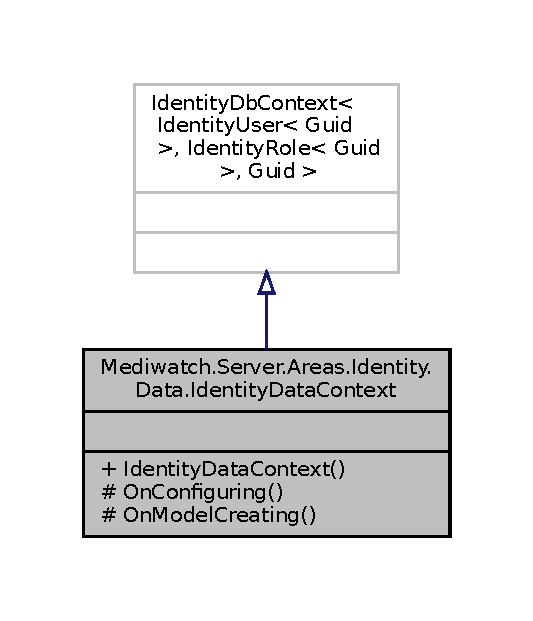
\includegraphics[width=242pt]{class_mediwatch_1_1_server_1_1_areas_1_1_identity_1_1_data_1_1_identity_data_context__inherit__graph}
\end{center}
\end{figure}


Graphe de collaboration de Mediwatch.\+Server.\+Areas.\+Identity.\+Data.\+Identity\+Data\+Context\+:\nopagebreak
\begin{figure}[H]
\begin{center}
\leavevmode
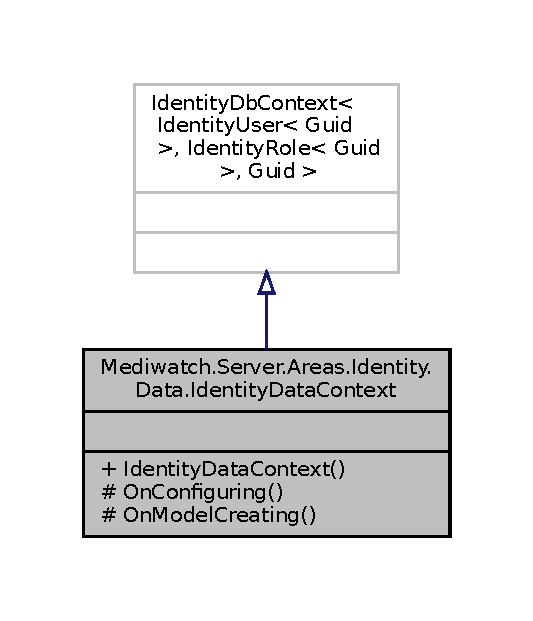
\includegraphics[width=242pt]{class_mediwatch_1_1_server_1_1_areas_1_1_identity_1_1_data_1_1_identity_data_context__coll__graph}
\end{center}
\end{figure}
\subsection*{Fonctions membres publiques}
\begin{DoxyCompactItemize}
\item 
\mbox{\Hypertarget{class_mediwatch_1_1_server_1_1_areas_1_1_identity_1_1_data_1_1_identity_data_context_ace53da6e49b7d2dff2bb67aad43cfa65}\label{class_mediwatch_1_1_server_1_1_areas_1_1_identity_1_1_data_1_1_identity_data_context_ace53da6e49b7d2dff2bb67aad43cfa65}} 
{\bfseries Identity\+Data\+Context} (Db\+Context\+Options$<$ \hyperlink{class_mediwatch_1_1_server_1_1_areas_1_1_identity_1_1_data_1_1_identity_data_context}{Identity\+Data\+Context} $>$ options)
\end{DoxyCompactItemize}
\subsection*{Fonctions membres protégées}
\begin{DoxyCompactItemize}
\item 
\mbox{\Hypertarget{class_mediwatch_1_1_server_1_1_areas_1_1_identity_1_1_data_1_1_identity_data_context_aa038bee1336ce8e66954bc5cfdc52e7a}\label{class_mediwatch_1_1_server_1_1_areas_1_1_identity_1_1_data_1_1_identity_data_context_aa038bee1336ce8e66954bc5cfdc52e7a}} 
override void {\bfseries On\+Model\+Creating} (Model\+Builder builder)
\end{DoxyCompactItemize}


La documentation de cette classe a été générée à partir du fichier suivant \+:\begin{DoxyCompactItemize}
\item 
Server/\+Areas/\+Identity/\+Data/Identity\+Data\+Context.\+cs\end{DoxyCompactItemize}

\hypertarget{class_mediwatch_1_1_server_1_1_migrations_1_1_identity_data_1_1_identity_data_context_model_snapshot}{}\section{Référence de la classe Mediwatch.\+Server.\+Migrations.\+Identity\+Data.\+Identity\+Data\+Context\+Model\+Snapshot}
\label{class_mediwatch_1_1_server_1_1_migrations_1_1_identity_data_1_1_identity_data_context_model_snapshot}\index{Mediwatch.\+Server.\+Migrations.\+Identity\+Data.\+Identity\+Data\+Context\+Model\+Snapshot@{Mediwatch.\+Server.\+Migrations.\+Identity\+Data.\+Identity\+Data\+Context\+Model\+Snapshot}}


Graphe d\textquotesingle{}héritage de Mediwatch.\+Server.\+Migrations.\+Identity\+Data.\+Identity\+Data\+Context\+Model\+Snapshot\+:\nopagebreak
\begin{figure}[H]
\begin{center}
\leavevmode
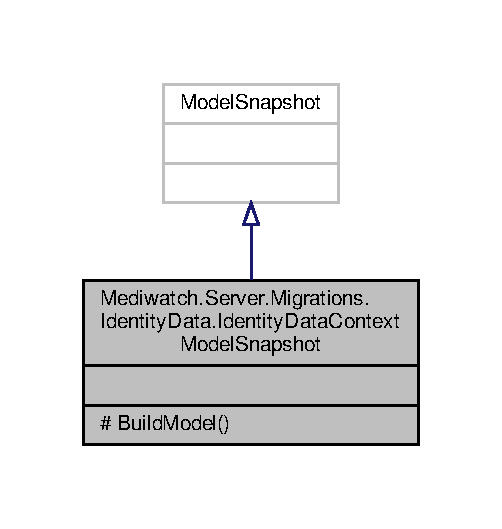
\includegraphics[width=241pt]{class_mediwatch_1_1_server_1_1_migrations_1_1_identity_data_1_1_identity_data_context_model_snapshot__inherit__graph}
\end{center}
\end{figure}


Graphe de collaboration de Mediwatch.\+Server.\+Migrations.\+Identity\+Data.\+Identity\+Data\+Context\+Model\+Snapshot\+:\nopagebreak
\begin{figure}[H]
\begin{center}
\leavevmode
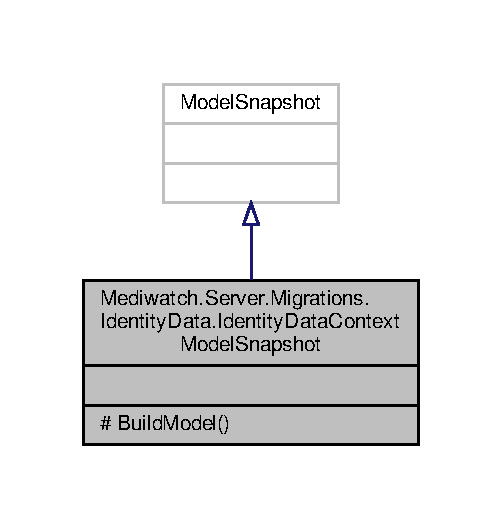
\includegraphics[width=241pt]{class_mediwatch_1_1_server_1_1_migrations_1_1_identity_data_1_1_identity_data_context_model_snapshot__coll__graph}
\end{center}
\end{figure}
\subsection*{Fonctions membres protégées}
\begin{DoxyCompactItemize}
\item 
\mbox{\Hypertarget{class_mediwatch_1_1_server_1_1_migrations_1_1_identity_data_1_1_identity_data_context_model_snapshot_ace9e9c05682cf740c45eeef4862fa09d}\label{class_mediwatch_1_1_server_1_1_migrations_1_1_identity_data_1_1_identity_data_context_model_snapshot_ace9e9c05682cf740c45eeef4862fa09d}} 
override void {\bfseries Build\+Model} (Model\+Builder model\+Builder)
\end{DoxyCompactItemize}


La documentation de cette classe a été générée à partir du fichier suivant \+:\begin{DoxyCompactItemize}
\item 
Server/\+Migrations/\+Identity\+Data/Identity\+Data\+Context\+Model\+Snapshot.\+cs\end{DoxyCompactItemize}

\hypertarget{class_mediwatch_1_1_server_1_1_areas_1_1_identity_1_1_identity_hosting_startup}{}\doxysection{Référence de la classe Mediwatch.\+Server.\+Areas.\+Identity.\+Identity\+Hosting\+Startup}
\label{class_mediwatch_1_1_server_1_1_areas_1_1_identity_1_1_identity_hosting_startup}\index{Mediwatch.Server.Areas.Identity.IdentityHostingStartup@{Mediwatch.Server.Areas.Identity.IdentityHostingStartup}}


Graphe d\textquotesingle{}héritage de Mediwatch.\+Server.\+Areas.\+Identity.\+Identity\+Hosting\+Startup\+:
\nopagebreak
\begin{figure}[H]
\begin{center}
\leavevmode
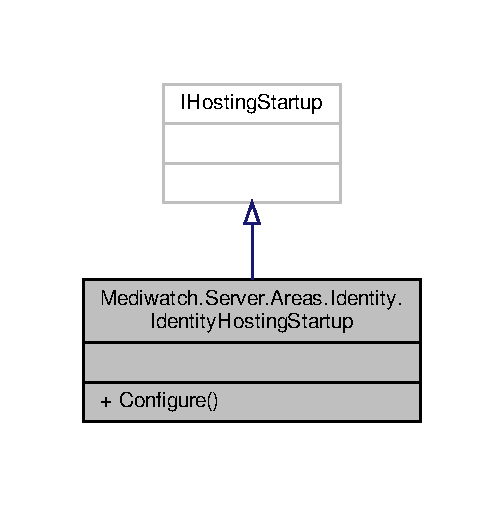
\includegraphics[width=256pt]{class_mediwatch_1_1_server_1_1_areas_1_1_identity_1_1_identity_hosting_startup__inherit__graph}
\end{center}
\end{figure}


Graphe de collaboration de Mediwatch.\+Server.\+Areas.\+Identity.\+Identity\+Hosting\+Startup\+:
\nopagebreak
\begin{figure}[H]
\begin{center}
\leavevmode
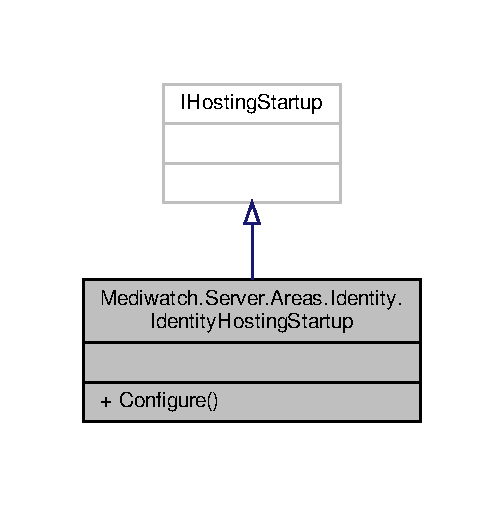
\includegraphics[width=256pt]{class_mediwatch_1_1_server_1_1_areas_1_1_identity_1_1_identity_hosting_startup__coll__graph}
\end{center}
\end{figure}
\doxysubsection*{Fonctions membres publiques}
\begin{DoxyCompactItemize}
\item 
\mbox{\Hypertarget{class_mediwatch_1_1_server_1_1_areas_1_1_identity_1_1_identity_hosting_startup_a4206ebb6e9389e9fee2397a1454f7f9b}\label{class_mediwatch_1_1_server_1_1_areas_1_1_identity_1_1_identity_hosting_startup_a4206ebb6e9389e9fee2397a1454f7f9b}} 
void {\bfseries Configure} (I\+Web\+Host\+Builder builder)
\end{DoxyCompactItemize}


La documentation de cette classe a été générée à partir du fichier suivant \+:\begin{DoxyCompactItemize}
\item 
Server/\+Areas/\+Identity/Identity\+Hosting\+Startup.\+cs\end{DoxyCompactItemize}

\hypertarget{class_mediwatch_1_1_server_1_1_migrations_1_1_migration_change_id_user}{}\section{Référence de la classe Mediwatch.\+Server.\+Migrations.\+Migration\+Change\+Id\+User}
\label{class_mediwatch_1_1_server_1_1_migrations_1_1_migration_change_id_user}\index{Mediwatch.\+Server.\+Migrations.\+Migration\+Change\+Id\+User@{Mediwatch.\+Server.\+Migrations.\+Migration\+Change\+Id\+User}}


Graphe d\textquotesingle{}héritage de Mediwatch.\+Server.\+Migrations.\+Migration\+Change\+Id\+User\+:\nopagebreak
\begin{figure}[H]
\begin{center}
\leavevmode
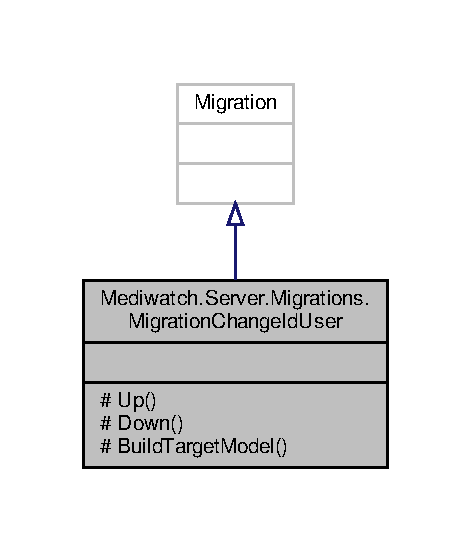
\includegraphics[width=226pt]{class_mediwatch_1_1_server_1_1_migrations_1_1_migration_change_id_user__inherit__graph}
\end{center}
\end{figure}


Graphe de collaboration de Mediwatch.\+Server.\+Migrations.\+Migration\+Change\+Id\+User\+:\nopagebreak
\begin{figure}[H]
\begin{center}
\leavevmode
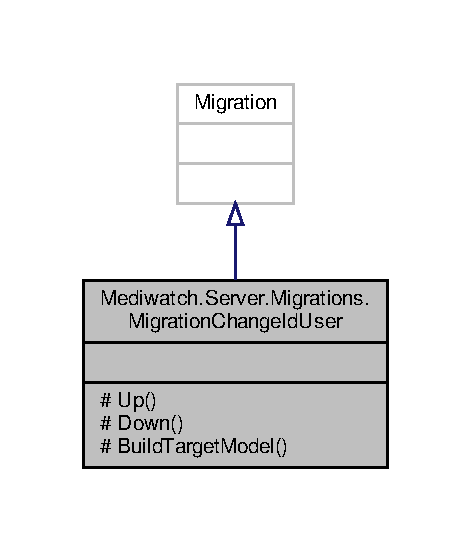
\includegraphics[width=226pt]{class_mediwatch_1_1_server_1_1_migrations_1_1_migration_change_id_user__coll__graph}
\end{center}
\end{figure}
\subsection*{Fonctions membres protégées}
\begin{DoxyCompactItemize}
\item 
\mbox{\Hypertarget{class_mediwatch_1_1_server_1_1_migrations_1_1_migration_change_id_user_a5416ab1301818531fae0a3bc3704f9ce}\label{class_mediwatch_1_1_server_1_1_migrations_1_1_migration_change_id_user_a5416ab1301818531fae0a3bc3704f9ce}} 
override void {\bfseries Up} (Migration\+Builder migration\+Builder)
\item 
\mbox{\Hypertarget{class_mediwatch_1_1_server_1_1_migrations_1_1_migration_change_id_user_a86f497448b9e0a91e2aba2be4a183a4b}\label{class_mediwatch_1_1_server_1_1_migrations_1_1_migration_change_id_user_a86f497448b9e0a91e2aba2be4a183a4b}} 
override void {\bfseries Down} (Migration\+Builder migration\+Builder)
\item 
\mbox{\Hypertarget{class_mediwatch_1_1_server_1_1_migrations_1_1_migration_change_id_user_a1bf8d925640d36f0d81655e4a6054e9b}\label{class_mediwatch_1_1_server_1_1_migrations_1_1_migration_change_id_user_a1bf8d925640d36f0d81655e4a6054e9b}} 
override void {\bfseries Build\+Target\+Model} (Model\+Builder model\+Builder)
\end{DoxyCompactItemize}


La documentation de cette classe a été générée à partir des fichiers suivants \+:\begin{DoxyCompactItemize}
\item 
Server/\+Migrations/20201224152510\+\_\+\+Migration\+Change\+Id\+User.\+cs\item 
Server/\+Migrations/20201224152510\+\_\+\+Migration\+Change\+Id\+User.\+Designer.\+cs\end{DoxyCompactItemize}

\hypertarget{class_mediwatch_1_1_server_1_1_program}{}\doxysection{Référence de la classe Mediwatch.\+Server.\+Program}
\label{class_mediwatch_1_1_server_1_1_program}\index{Mediwatch.Server.Program@{Mediwatch.Server.Program}}


Graphe de collaboration de Mediwatch.\+Server.\+Program\+:
% FIG 0
\doxysubsection*{Fonctions membres publiques statiques}
\begin{DoxyCompactItemize}
\item 
static void \mbox{\hyperlink{class_mediwatch_1_1_server_1_1_program_a0b37e08654729aa1c9f3a572e5775305}{Main}} (string\mbox{[}$\,$\mbox{]} args)
\item 
static I\+Host\+Builder \mbox{\hyperlink{class_mediwatch_1_1_server_1_1_program_a5278302328dd5740238221820ef8fa07}{Create\+Host\+Builder}} (string\mbox{[}$\,$\mbox{]} args)
\end{DoxyCompactItemize}


\doxysubsection{Documentation des fonctions membres}
\mbox{\Hypertarget{class_mediwatch_1_1_server_1_1_program_a5278302328dd5740238221820ef8fa07}\label{class_mediwatch_1_1_server_1_1_program_a5278302328dd5740238221820ef8fa07}} 
\index{Mediwatch.Server.Program@{Mediwatch.Server.Program}!CreateHostBuilder@{CreateHostBuilder}}
\index{CreateHostBuilder@{CreateHostBuilder}!Mediwatch.Server.Program@{Mediwatch.Server.Program}}
\doxysubsubsection{\texorpdfstring{CreateHostBuilder()}{CreateHostBuilder()}}
{\footnotesize\ttfamily static I\+Host\+Builder Mediwatch.\+Server.\+Program.\+Create\+Host\+Builder (\begin{DoxyParamCaption}\item[{string\mbox{[}$\,$\mbox{]}}]{args }\end{DoxyParamCaption})\hspace{0.3cm}{\ttfamily [static]}}

\mbox{\Hypertarget{class_mediwatch_1_1_server_1_1_program_a0b37e08654729aa1c9f3a572e5775305}\label{class_mediwatch_1_1_server_1_1_program_a0b37e08654729aa1c9f3a572e5775305}} 
\index{Mediwatch.Server.Program@{Mediwatch.Server.Program}!Main@{Main}}
\index{Main@{Main}!Mediwatch.Server.Program@{Mediwatch.Server.Program}}
\doxysubsubsection{\texorpdfstring{Main()}{Main()}}
{\footnotesize\ttfamily static void Mediwatch.\+Server.\+Program.\+Main (\begin{DoxyParamCaption}\item[{string\mbox{[}$\,$\mbox{]}}]{args }\end{DoxyParamCaption})\hspace{0.3cm}{\ttfamily [static]}}



La documentation de cette classe a été générée à partir du fichier suivant \+:\begin{DoxyCompactItemize}
\item 
Server/\mbox{\hyperlink{_program_8cs}{Program.\+cs}}\end{DoxyCompactItemize}

\hypertarget{class_mediwatch_1_1_server_1_1_startup}{}\section{Référence de la classe Mediwatch.\+Server.\+Startup}
\label{class_mediwatch_1_1_server_1_1_startup}\index{Mediwatch.\+Server.\+Startup@{Mediwatch.\+Server.\+Startup}}


Graphe de collaboration de Mediwatch.\+Server.\+Startup\+:
\nopagebreak
\begin{figure}[H]
\begin{center}
\leavevmode
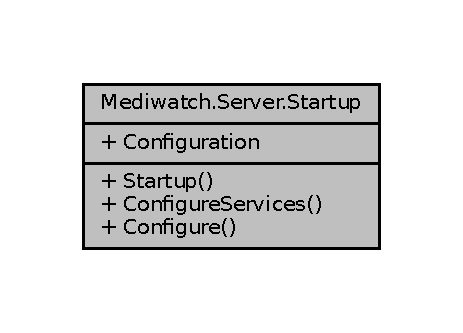
\includegraphics[width=210pt]{class_mediwatch_1_1_server_1_1_startup__coll__graph}
\end{center}
\end{figure}
\subsection*{Fonctions membres publiques}
\begin{DoxyCompactItemize}
\item 
\mbox{\Hypertarget{class_mediwatch_1_1_server_1_1_startup_a99779cbd7c184cbff98730a5f285a647}\label{class_mediwatch_1_1_server_1_1_startup_a99779cbd7c184cbff98730a5f285a647}} 
{\bfseries Startup} (I\+Configuration configuration)
\item 
\mbox{\Hypertarget{class_mediwatch_1_1_server_1_1_startup_a98b7f4b5e49a83c353687ec3c1cfa139}\label{class_mediwatch_1_1_server_1_1_startup_a98b7f4b5e49a83c353687ec3c1cfa139}} 
void {\bfseries Configure\+Services} (I\+Service\+Collection services)
\item 
\mbox{\Hypertarget{class_mediwatch_1_1_server_1_1_startup_af31b63124f79f812e79cb6f43df14a40}\label{class_mediwatch_1_1_server_1_1_startup_af31b63124f79f812e79cb6f43df14a40}} 
void {\bfseries Configure} (I\+Application\+Builder app, I\+Web\+Host\+Environment env)
\end{DoxyCompactItemize}
\subsection*{Propriétés}
\begin{DoxyCompactItemize}
\item 
\mbox{\Hypertarget{class_mediwatch_1_1_server_1_1_startup_ae3d0512feacc2872ab0ec4d5082626a6}\label{class_mediwatch_1_1_server_1_1_startup_ae3d0512feacc2872ab0ec4d5082626a6}} 
I\+Configuration {\bfseries Configuration}\hspace{0.3cm}{\ttfamily  \mbox{[}get\mbox{]}}
\end{DoxyCompactItemize}


La documentation de cette classe a été générée à partir du fichier suivant \+:\begin{DoxyCompactItemize}
\item 
Server/Startup.\+cs\end{DoxyCompactItemize}

\hypertarget{class_mediwatch_1_1_server_1_1_migrations_1_1_identity_data_1_1_user_role}{}\section{Référence de la classe Mediwatch.\+Server.\+Migrations.\+Identity\+Data.\+User\+Role}
\label{class_mediwatch_1_1_server_1_1_migrations_1_1_identity_data_1_1_user_role}\index{Mediwatch.\+Server.\+Migrations.\+Identity\+Data.\+User\+Role@{Mediwatch.\+Server.\+Migrations.\+Identity\+Data.\+User\+Role}}


Graphe d\textquotesingle{}héritage de Mediwatch.\+Server.\+Migrations.\+Identity\+Data.\+User\+Role\+:\nopagebreak
\begin{figure}[H]
\begin{center}
\leavevmode
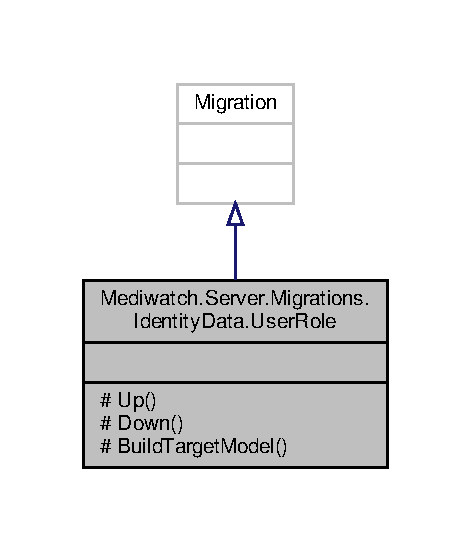
\includegraphics[width=226pt]{class_mediwatch_1_1_server_1_1_migrations_1_1_identity_data_1_1_user_role__inherit__graph}
\end{center}
\end{figure}


Graphe de collaboration de Mediwatch.\+Server.\+Migrations.\+Identity\+Data.\+User\+Role\+:\nopagebreak
\begin{figure}[H]
\begin{center}
\leavevmode
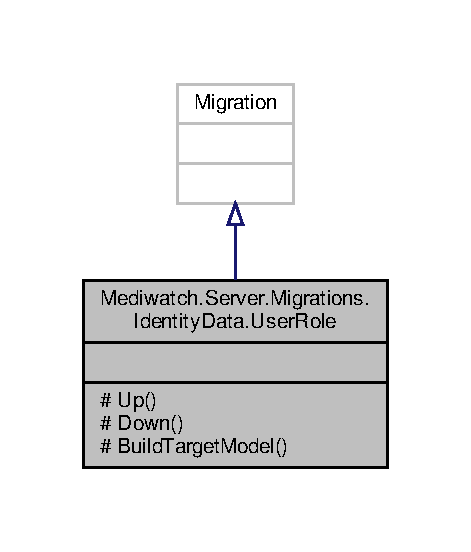
\includegraphics[width=226pt]{class_mediwatch_1_1_server_1_1_migrations_1_1_identity_data_1_1_user_role__coll__graph}
\end{center}
\end{figure}
\subsection*{Fonctions membres protégées}
\begin{DoxyCompactItemize}
\item 
\mbox{\Hypertarget{class_mediwatch_1_1_server_1_1_migrations_1_1_identity_data_1_1_user_role_a8ccaaaabfb6492822c891a222ea9146e}\label{class_mediwatch_1_1_server_1_1_migrations_1_1_identity_data_1_1_user_role_a8ccaaaabfb6492822c891a222ea9146e}} 
override void {\bfseries Up} (Migration\+Builder migration\+Builder)
\item 
\mbox{\Hypertarget{class_mediwatch_1_1_server_1_1_migrations_1_1_identity_data_1_1_user_role_a37c0913be87d41042398bbc9127e7300}\label{class_mediwatch_1_1_server_1_1_migrations_1_1_identity_data_1_1_user_role_a37c0913be87d41042398bbc9127e7300}} 
override void {\bfseries Down} (Migration\+Builder migration\+Builder)
\item 
\mbox{\Hypertarget{class_mediwatch_1_1_server_1_1_migrations_1_1_identity_data_1_1_user_role_a43904c2791341bd27330059634f3a01b}\label{class_mediwatch_1_1_server_1_1_migrations_1_1_identity_data_1_1_user_role_a43904c2791341bd27330059634f3a01b}} 
override void {\bfseries Build\+Target\+Model} (Model\+Builder model\+Builder)
\end{DoxyCompactItemize}


La documentation de cette classe a été générée à partir des fichiers suivants \+:\begin{DoxyCompactItemize}
\item 
Server/\+Migrations/\+Identity\+Data/20201224152723\+\_\+\+User\+Role.\+cs\item 
Server/\+Migrations/\+Identity\+Data/20201224152723\+\_\+\+User\+Role.\+Designer.\+cs\end{DoxyCompactItemize}

\hypertarget{class_mediwatch_1_1_server_1_1_controllers_1_1_users_controller}{}\doxysection{Référence de la classe Mediwatch.\+Server.\+Controllers.\+Users\+Controller}
\label{class_mediwatch_1_1_server_1_1_controllers_1_1_users_controller}\index{Mediwatch.Server.Controllers.UsersController@{Mediwatch.Server.Controllers.UsersController}}


Graphe d\textquotesingle{}héritage de Mediwatch.\+Server.\+Controllers.\+Users\+Controller\+:\nopagebreak
\begin{figure}[H]
\begin{center}
\leavevmode
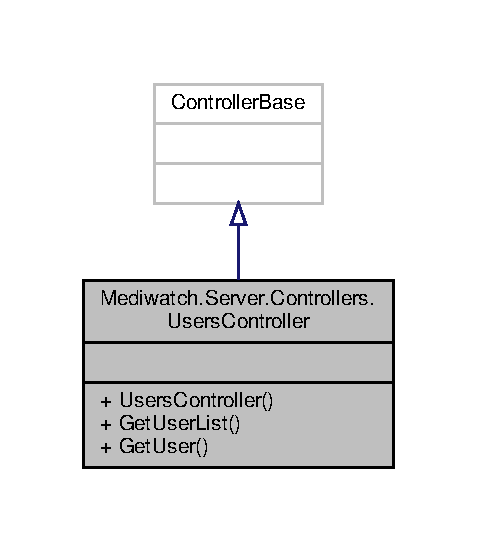
\includegraphics[width=243pt]{class_mediwatch_1_1_server_1_1_controllers_1_1_users_controller__inherit__graph}
\end{center}
\end{figure}


Graphe de collaboration de Mediwatch.\+Server.\+Controllers.\+Users\+Controller\+:\nopagebreak
\begin{figure}[H]
\begin{center}
\leavevmode
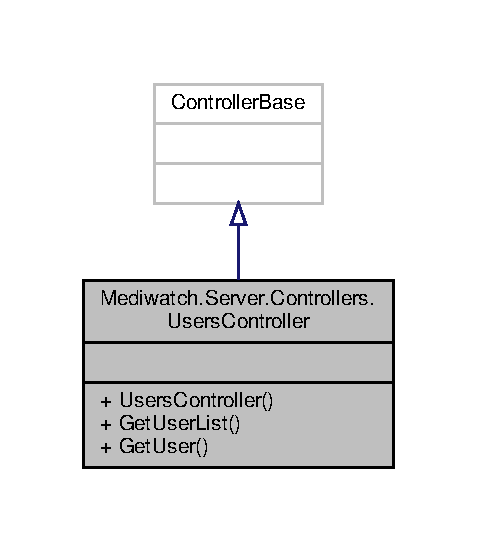
\includegraphics[width=243pt]{class_mediwatch_1_1_server_1_1_controllers_1_1_users_controller__coll__graph}
\end{center}
\end{figure}
\doxysubsection*{Fonctions membres publiques}
\begin{DoxyCompactItemize}
\item 
\mbox{\Hypertarget{class_mediwatch_1_1_server_1_1_controllers_1_1_users_controller_af805109a035bb309ea173491e8674812}\label{class_mediwatch_1_1_server_1_1_controllers_1_1_users_controller_af805109a035bb309ea173491e8674812}} 
{\bfseries Users\+Controller} (User\+Manager$<$ \mbox{\hyperlink{class_mediwatch_1_1_server_1_1_areas_1_1_identity_1_1_data_1_1_user_custom}{User\+Custom}} $>$ user\+Manager, \mbox{\hyperlink{class_server_1_1_db_context_mediwatch}{Db\+Context\+Mediwatch}} context)
\item 
async Task$<$ Action\+Result$<$ I\+Enumerable$<$ User\+Public $>$ $>$ $>$ \mbox{\hyperlink{class_mediwatch_1_1_server_1_1_controllers_1_1_users_controller_a5b525adc63d36869bde5021b82480228}{Get\+User\+List}} ()
\begin{DoxyCompactList}\small\item\em list all users if you are admin G\+ET\+: /\+Users/list\+User \end{DoxyCompactList}\item 
async Task$<$ Action\+Result$<$ User\+Public $>$ $>$ \mbox{\hyperlink{class_mediwatch_1_1_server_1_1_controllers_1_1_users_controller_a9a705b16c851ce5bb20f426b6e923799}{Get\+My\+User}} ()
\begin{DoxyCompactList}\small\item\em Get the information of the connected user A\+PI G\+ET \+: /\+Users/info \end{DoxyCompactList}\item 
async Task$<$ Action\+Result$<$ User\+Public $>$ $>$ \mbox{\hyperlink{class_mediwatch_1_1_server_1_1_controllers_1_1_users_controller_a27103389ca1c6c33d21a3dc3212d7b08}{Get\+User}} (String id)
\begin{DoxyCompactList}\small\item\em get info of one user G\+ET\+: /\+Users/info/\{id user\} \end{DoxyCompactList}\item 
async Task$<$ Action\+Result $>$ \mbox{\hyperlink{class_mediwatch_1_1_server_1_1_controllers_1_1_users_controller_a414ca2854bf71701319b3c34dbda03ab}{Set\+User}} (User\+Public user)
\begin{DoxyCompactList}\small\item\em set info of one user P\+O\+ST\+: /\+Users/set\+Info/ B\+O\+DY\+: raw/json \+:User\+Public \end{DoxyCompactList}\item 
async Task$<$ Action\+Result$<$ I\+Enumerable$<$ applicant\+\_\+session $>$ $>$ $>$ \mbox{\hyperlink{class_mediwatch_1_1_server_1_1_controllers_1_1_users_controller_a3da0476c39418727064b44af9e007010}{Get\+User\+Formation}} (String id)
\begin{DoxyCompactList}\small\item\em G\+ET\+: /\+Users/formation/\{id user\} get all formation of one user \end{DoxyCompactList}\item 
async Task$<$ Action\+Result$<$ applicant\+\_\+session $>$ $>$ \mbox{\hyperlink{class_mediwatch_1_1_server_1_1_controllers_1_1_users_controller_a44bf781dad67f766e1d0c91ac17d73ef}{Register\+Userformation}} (applicant\+\_\+session Register\+User)
\begin{DoxyCompactList}\small\item\em P\+O\+ST\+: /\+Users/registeruserformation/ B\+O\+DY\+: raw/json \+:applicant\+\_\+session, create register user to a Formation \end{DoxyCompactList}\item 
async Task$<$ Action\+Result$<$ applicant\+\_\+session $>$ $>$ \mbox{\hyperlink{class_mediwatch_1_1_server_1_1_controllers_1_1_users_controller_a03952b3be592e56eb93c7c6abdfe297b}{Delete\+User\+Formation}} (applicant\+\_\+session body)
\begin{DoxyCompactList}\small\item\em D\+EL\+: /\+Users/deleteuserformation/ B\+O\+DY\+: raw/json \+:applicant\+\_\+session, with id Applicant\+Session and Id\+Formation create register user to a Formation \end{DoxyCompactList}\end{DoxyCompactItemize}


\doxysubsection{Documentation des fonctions membres}
\mbox{\Hypertarget{class_mediwatch_1_1_server_1_1_controllers_1_1_users_controller_a03952b3be592e56eb93c7c6abdfe297b}\label{class_mediwatch_1_1_server_1_1_controllers_1_1_users_controller_a03952b3be592e56eb93c7c6abdfe297b}} 
\index{Mediwatch.Server.Controllers.UsersController@{Mediwatch.Server.Controllers.UsersController}!DeleteUserFormation@{DeleteUserFormation}}
\index{DeleteUserFormation@{DeleteUserFormation}!Mediwatch.Server.Controllers.UsersController@{Mediwatch.Server.Controllers.UsersController}}
\doxysubsubsection{\texorpdfstring{DeleteUserFormation()}{DeleteUserFormation()}}
{\footnotesize\ttfamily async Task$<$Action\+Result$<$applicant\+\_\+session$>$ $>$ Mediwatch.\+Server.\+Controllers.\+Users\+Controller.\+Delete\+User\+Formation (\begin{DoxyParamCaption}\item[{applicant\+\_\+session}]{body }\end{DoxyParamCaption})\hspace{0.3cm}{\ttfamily [inline]}}



D\+EL\+: /\+Users/deleteuserformation/ B\+O\+DY\+: raw/json \+:applicant\+\_\+session, with id Applicant\+Session and Id\+Formation create register user to a Formation 


\begin{DoxyParams}{Paramètres}
{\em body.\+id} & id of the applicant\+Session\\
\hline
{\em body.\+id\+User} & id\+User of the applicant\+Session\\
\hline
\end{DoxyParams}
\begin{DoxyReturn}{Renvoie}
return one applicant session
\end{DoxyReturn}
\mbox{\Hypertarget{class_mediwatch_1_1_server_1_1_controllers_1_1_users_controller_a9a705b16c851ce5bb20f426b6e923799}\label{class_mediwatch_1_1_server_1_1_controllers_1_1_users_controller_a9a705b16c851ce5bb20f426b6e923799}} 
\index{Mediwatch.Server.Controllers.UsersController@{Mediwatch.Server.Controllers.UsersController}!GetMyUser@{GetMyUser}}
\index{GetMyUser@{GetMyUser}!Mediwatch.Server.Controllers.UsersController@{Mediwatch.Server.Controllers.UsersController}}
\doxysubsubsection{\texorpdfstring{GetMyUser()}{GetMyUser()}}
{\footnotesize\ttfamily async Task$<$Action\+Result$<$User\+Public$>$ $>$ Mediwatch.\+Server.\+Controllers.\+Users\+Controller.\+Get\+My\+User (\begin{DoxyParamCaption}{ }\end{DoxyParamCaption})\hspace{0.3cm}{\ttfamily [inline]}}



Get the information of the connected user A\+PI G\+ET \+: /\+Users/info 

\begin{DoxyReturn}{Renvoie}
return a user public user with the information of the connected user
\end{DoxyReturn}
\mbox{\Hypertarget{class_mediwatch_1_1_server_1_1_controllers_1_1_users_controller_a27103389ca1c6c33d21a3dc3212d7b08}\label{class_mediwatch_1_1_server_1_1_controllers_1_1_users_controller_a27103389ca1c6c33d21a3dc3212d7b08}} 
\index{Mediwatch.Server.Controllers.UsersController@{Mediwatch.Server.Controllers.UsersController}!GetUser@{GetUser}}
\index{GetUser@{GetUser}!Mediwatch.Server.Controllers.UsersController@{Mediwatch.Server.Controllers.UsersController}}
\doxysubsubsection{\texorpdfstring{GetUser()}{GetUser()}}
{\footnotesize\ttfamily async Task$<$Action\+Result$<$User\+Public$>$ $>$ Mediwatch.\+Server.\+Controllers.\+Users\+Controller.\+Get\+User (\begin{DoxyParamCaption}\item[{String}]{id }\end{DoxyParamCaption})\hspace{0.3cm}{\ttfamily [inline]}}



get info of one user G\+ET\+: /\+Users/info/\{id user\} 


\begin{DoxyParams}{Paramètres}
{\em id} & the id of the user\\
\hline
\end{DoxyParams}
\begin{DoxyReturn}{Renvoie}
return a user public if the id correspond to the id of the connected user. Return not found in case of not base 64 id, the id is not found in the data base or if you\textquotesingle{}re not admin else it will return a user public with the information corresponding to the user id
\end{DoxyReturn}
\mbox{\Hypertarget{class_mediwatch_1_1_server_1_1_controllers_1_1_users_controller_a3da0476c39418727064b44af9e007010}\label{class_mediwatch_1_1_server_1_1_controllers_1_1_users_controller_a3da0476c39418727064b44af9e007010}} 
\index{Mediwatch.Server.Controllers.UsersController@{Mediwatch.Server.Controllers.UsersController}!GetUserFormation@{GetUserFormation}}
\index{GetUserFormation@{GetUserFormation}!Mediwatch.Server.Controllers.UsersController@{Mediwatch.Server.Controllers.UsersController}}
\doxysubsubsection{\texorpdfstring{GetUserFormation()}{GetUserFormation()}}
{\footnotesize\ttfamily async Task$<$Action\+Result$<$I\+Enumerable$<$applicant\+\_\+session$>$ $>$ $>$ Mediwatch.\+Server.\+Controllers.\+Users\+Controller.\+Get\+User\+Formation (\begin{DoxyParamCaption}\item[{String}]{id }\end{DoxyParamCaption})\hspace{0.3cm}{\ttfamily [inline]}}



G\+ET\+: /\+Users/formation/\{id user\} get all formation of one user 


\begin{DoxyParams}{Paramètres}
{\em id} & id user\\
\hline
\end{DoxyParams}
\begin{DoxyReturn}{Renvoie}
return the list of applicant session
\end{DoxyReturn}
\mbox{\Hypertarget{class_mediwatch_1_1_server_1_1_controllers_1_1_users_controller_a5b525adc63d36869bde5021b82480228}\label{class_mediwatch_1_1_server_1_1_controllers_1_1_users_controller_a5b525adc63d36869bde5021b82480228}} 
\index{Mediwatch.Server.Controllers.UsersController@{Mediwatch.Server.Controllers.UsersController}!GetUserList@{GetUserList}}
\index{GetUserList@{GetUserList}!Mediwatch.Server.Controllers.UsersController@{Mediwatch.Server.Controllers.UsersController}}
\doxysubsubsection{\texorpdfstring{GetUserList()}{GetUserList()}}
{\footnotesize\ttfamily async Task$<$Action\+Result$<$I\+Enumerable$<$User\+Public$>$ $>$ $>$ Mediwatch.\+Server.\+Controllers.\+Users\+Controller.\+Get\+User\+List (\begin{DoxyParamCaption}{ }\end{DoxyParamCaption})\hspace{0.3cm}{\ttfamily [inline]}}



list all users if you are admin G\+ET\+: /\+Users/list\+User 

\begin{DoxyReturn}{Renvoie}
return unauthorized if the user role is not admin and a list of public user when it work
\end{DoxyReturn}
\mbox{\Hypertarget{class_mediwatch_1_1_server_1_1_controllers_1_1_users_controller_a44bf781dad67f766e1d0c91ac17d73ef}\label{class_mediwatch_1_1_server_1_1_controllers_1_1_users_controller_a44bf781dad67f766e1d0c91ac17d73ef}} 
\index{Mediwatch.Server.Controllers.UsersController@{Mediwatch.Server.Controllers.UsersController}!RegisterUserformation@{RegisterUserformation}}
\index{RegisterUserformation@{RegisterUserformation}!Mediwatch.Server.Controllers.UsersController@{Mediwatch.Server.Controllers.UsersController}}
\doxysubsubsection{\texorpdfstring{RegisterUserformation()}{RegisterUserformation()}}
{\footnotesize\ttfamily async Task$<$Action\+Result$<$applicant\+\_\+session$>$ $>$ Mediwatch.\+Server.\+Controllers.\+Users\+Controller.\+Register\+Userformation (\begin{DoxyParamCaption}\item[{applicant\+\_\+session}]{Register\+User }\end{DoxyParamCaption})\hspace{0.3cm}{\ttfamily [inline]}}



P\+O\+ST\+: /\+Users/registeruserformation/ B\+O\+DY\+: raw/json \+:applicant\+\_\+session, create register user to a Formation 


\begin{DoxyParams}{Paramètres}
{\em id\+Formation} & id of the formation\\
\hline
\end{DoxyParams}
\begin{DoxyReturn}{Renvoie}
return one applicant session
\end{DoxyReturn}
\mbox{\Hypertarget{class_mediwatch_1_1_server_1_1_controllers_1_1_users_controller_a414ca2854bf71701319b3c34dbda03ab}\label{class_mediwatch_1_1_server_1_1_controllers_1_1_users_controller_a414ca2854bf71701319b3c34dbda03ab}} 
\index{Mediwatch.Server.Controllers.UsersController@{Mediwatch.Server.Controllers.UsersController}!SetUser@{SetUser}}
\index{SetUser@{SetUser}!Mediwatch.Server.Controllers.UsersController@{Mediwatch.Server.Controllers.UsersController}}
\doxysubsubsection{\texorpdfstring{SetUser()}{SetUser()}}
{\footnotesize\ttfamily async Task$<$Action\+Result$>$ Mediwatch.\+Server.\+Controllers.\+Users\+Controller.\+Set\+User (\begin{DoxyParamCaption}\item[{User\+Public}]{user }\end{DoxyParamCaption})\hspace{0.3cm}{\ttfamily [inline]}}



set info of one user P\+O\+ST\+: /\+Users/set\+Info/ B\+O\+DY\+: raw/json \+:User\+Public 


\begin{DoxyParams}{Paramètres}
{\em user} & information to set\\
\hline
\end{DoxyParams}
\begin{DoxyReturn}{Renvoie}
return OK if the id correspond to the id of the connected user. Return not found in case of not base 64 id, the id is not found in the data base or if you\textquotesingle{}re not admin else it will return OK
\end{DoxyReturn}


La documentation de cette classe a été générée à partir du fichier suivant \+:\begin{DoxyCompactItemize}
\item 
Server/\+Controllers/Users\+Info\+Controller.\+cs\end{DoxyCompactItemize}

\hypertarget{class_mediwatch_1_1_server_1_1_controllers_1_1_weather_forecast_controller}{}\doxysection{Référence de la classe Mediwatch.\+Server.\+Controllers.\+Weather\+Forecast\+Controller}
\label{class_mediwatch_1_1_server_1_1_controllers_1_1_weather_forecast_controller}\index{Mediwatch.Server.Controllers.WeatherForecastController@{Mediwatch.Server.Controllers.WeatherForecastController}}


Graphe d\textquotesingle{}héritage de Mediwatch.\+Server.\+Controllers.\+Weather\+Forecast\+Controller\+:
\nopagebreak
\begin{figure}[H]
\begin{center}
\leavevmode
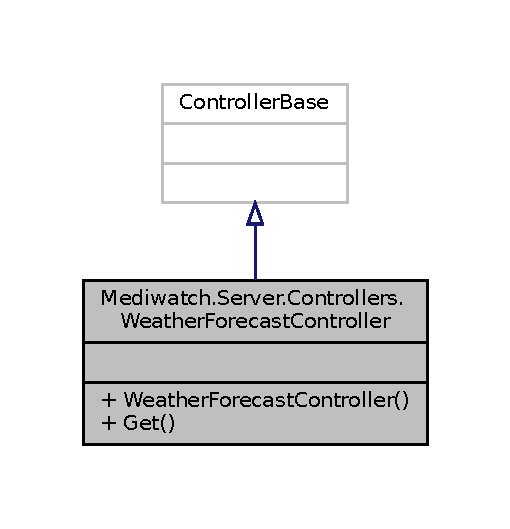
\includegraphics[width=245pt]{class_mediwatch_1_1_server_1_1_controllers_1_1_weather_forecast_controller__inherit__graph}
\end{center}
\end{figure}


Graphe de collaboration de Mediwatch.\+Server.\+Controllers.\+Weather\+Forecast\+Controller\+:
\nopagebreak
\begin{figure}[H]
\begin{center}
\leavevmode
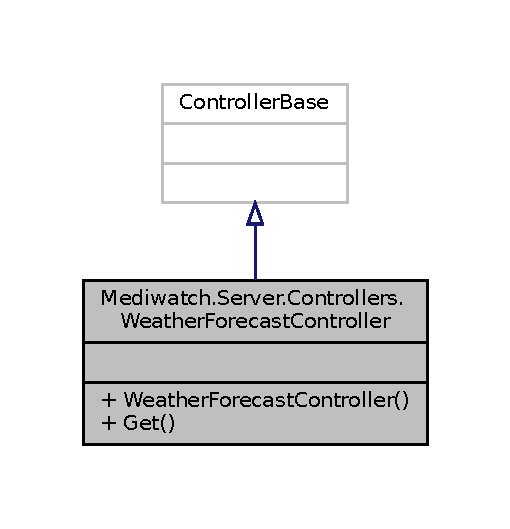
\includegraphics[width=245pt]{class_mediwatch_1_1_server_1_1_controllers_1_1_weather_forecast_controller__coll__graph}
\end{center}
\end{figure}
\doxysubsection*{Fonctions membres publiques}
\begin{DoxyCompactItemize}
\item 
\mbox{\Hypertarget{class_mediwatch_1_1_server_1_1_controllers_1_1_weather_forecast_controller_a8557f93a28d98c9487aa7c812cb61c18}\label{class_mediwatch_1_1_server_1_1_controllers_1_1_weather_forecast_controller_a8557f93a28d98c9487aa7c812cb61c18}} 
{\bfseries Weather\+Forecast\+Controller} (I\+Logger$<$ \mbox{\hyperlink{class_mediwatch_1_1_server_1_1_controllers_1_1_weather_forecast_controller}{Weather\+Forecast\+Controller}} $>$ logger)
\item 
\mbox{\Hypertarget{class_mediwatch_1_1_server_1_1_controllers_1_1_weather_forecast_controller_a43eaa75ecf6f43cba687aeb38a08636f}\label{class_mediwatch_1_1_server_1_1_controllers_1_1_weather_forecast_controller_a43eaa75ecf6f43cba687aeb38a08636f}} 
I\+Enumerable$<$ Weather\+Forecast $>$ {\bfseries Get} ()
\end{DoxyCompactItemize}


La documentation de cette classe a été générée à partir du fichier suivant \+:\begin{DoxyCompactItemize}
\item 
Server/\+Controllers/Weather\+Forecast\+Controller.\+cs\end{DoxyCompactItemize}

%--- End generated contents ---

% Index
\backmatter
\newpage
\phantomsection
\clearemptydoublepage
\addcontentsline{toc}{chapter}{Index}
\printindex

\end{document}
